\documentclass[11pt,a4paper]{report}

\usepackage{mathpazo}
\usepackage{microtype}
\usepackage{titlesec}
\usepackage{url}
\usepackage{hyperref}
\usepackage{verbatim}

\usepackage{tikz}
\usetikzlibrary{external,shapes.geometric}
%\tikzexternalize[prefix=tikz/]

\textwidth=15cm
\textheight=23cm
\topmargin=12pt
\headheight=0pt
\oddsidemargin=2em
\headsep=0pt
\renewcommand{\baselinestretch}{1.1}
\setlength{\parskip}{0.2\baselineskip plus 1pt minus 1pt}
\parindent=0pt

\titleformat{\chapter}[display]{\normalfont\huge\bfseries}{\chaptertitlename\ \thechapter}{10pt}{\Huge}   
\titlespacing*{\chapter}{0pt}{-20pt}{20pt}
\titleformat{\section}[block]{\normalfont\Large\bfseries}{\thesection}{8pt}{\Large}
\setcounter{tocdepth}{1}

\newcommand*{\p}[1]{\texttt{\textup{\footnotesize #1}}}
\newcommand*{\ih}{\stackrel{\bullet}{=}}
\newcommand*{\ihge}{\stackrel{\bullet}{\geq}}
\newcommand*{\ihlt}{\stackrel{\bullet}{<}}
\newcommand*{\ihle}{\stackrel{\bullet}{\leq}}
\newcommand*{\qeq}{\stackrel{?}{=}}
\newcommand*{\qge}{\stackrel{?}{\geq}}

\newcommand*{\qed}{\hfill\rule{1ex}{1.5ex}}
\newcommand*{\qedd}[1]{\vspace*{-#1ex}\qed}

\newtheorem{theorem}{Theorem}
\newtheorem{definition}[theorem]{Definition}
\newtheorem{axiom}{Axiom}
\newtheorem{lemma}[theorem]{Lemma}
\newtheorem{exercise}{Exercise}

\begin{document}
\thispagestyle{empty}

\begin{center}
\begin{Huge}
\begin{bfseries}
The Many Guises of Induction
\end{bfseries}
\end{Huge}

\bigskip
\bigskip
\bigskip

\textbf{\LARGE Moti Ben-Ari}

\bigskip

\textbf{\Large Department of Science Teaching\\
Weizmann Institute of Science\\
\bigskip
\url{http://www.weizmann.ac.il/sci-tea/benari/}
}

\bigskip
\bigskip


\begin{Large}
Version 1.6.0
\end{Large}
\end{center}

\vfill

\begin{center}
\copyright{}\  2016--19 by Moti Ben-Ari.
\end{center}

This work is licensed under the Creative Commons Attribution-ShareAlike 3.0 Unported License. To view a copy of this license, visit \url{http://creativecommons.org/licenses/by-sa/3.0/} or send a letter to Creative Commons, 444 Castro Street, Suite 900, Mountain View, California, 94041, USA.

\begin{center}
\includegraphics[width=.2\textwidth]{../../by-sa.png}
\end{center}

\newpage

\setcounter{tocdepth}{0}
\tableofcontents

\chapter{Introduction}\label{s.intro}

Induction is one of the most widely used proof techniques in mathematics to the extent that it is used routinely and often implicitly. A side effect of the routine use of induction is that it is frequently taught as a set of steps to be followed and not as a fundamental concept. This document presents a short course on induction that shows the richness of the concept and the different ways in which it appears in mathematics.

The presentation is broad rather than deep: the aim is to present induction in as many forms as possible, so only one or two examples and exercises are given for each topic, unlike a textbook with many examples and numerous exercises. The document is written at several levels: some parts are appropriate for advanced high-school students, while other parts are aimed at undergraduate students, and teachers of mathematics and computer science. Feel free to skip parts concerning topics you are not familiar with. 

Chapters~\ref{s.axiom}--\ref{s.watch} should be accessible to high school students. Chapter~\ref{s.axiom} is a rather long discourse intended to motivate the need for mathematical induction and to present it as an axiom. Chapter~\ref{s.integers} presents classical mathematical induction over the integers, with sections devoted to differences in the application of the axiom. Chapter~\ref{s.notjust} is extremely important because it shows that induction is a fundamental proof technique for mathematical constructs other than integers. Chapter~\ref{s.watch} presents pitfalls that you should watch out for: induction is not the only proof method, induction is not always an appropriate proof method, and incorrect proofs can result if the base case and inductive steps are not carefully coordinated.

Chapters~\ref{s.logic}--\ref{s.verif} present the use of induction in topics of undergraduate mathematics and computer science. Chapter~\ref{s.logic} discusses induction on the structure of formulas of mathematical logic, while Chapter~\ref{s.models} demonstrates the use of induction in automata and formal languages. Chapter~\ref{s.verif} goes beyond abstract structures to investigate the use of induction in verifying the correctness of computer programs.

Chapters~\ref{s.ind-ded}--\ref{s.well} discuss the philosophical and theoretical aspects of induction. Chapter~\ref{s.ind-ded} explains how the use of the term ``induction'' in mathematics clashes with its use in science. Chapter~\ref{s.well} shows how to prove the rule of mathematical induction if the well-ordering principle is taken as an axiom.

Chapter~\ref{s.conclusion} wraps up the course on induction.

Appendix~\ref{a.challenge} poses challenging problems that do not need advanced mathematics.

Solutions to the exercises are given in an Appendix~\ref{a.solutions}.

%%%%%%%%%%%%%%%%%%%%%%%%%%%%%%%%%%%%%%%%%%%%%%%%%%%%%%%%%%%%%%%%%%%

\chapter[Mathematical Induction: An Indispensable Axiom]{Mathematical Induction:\\An Indispensable Axiom}\label{s.axiom}

In this chapter, we motivate the use of mathematical induction, give a formal definition and explain its nature as an axiom.

\section{Why do we need induction?}\label{s.why}

Let's jump right into proving some theorems:

\begin{theorem}\label{t.odd}
Every odd integer $n\geq 3$ is prime.
\end{theorem}

\textbf{Proof} The numbers $3,5,7$ are prime. Therefore, every odd integer $n\geq 3$ is prime.\qed

\begin{theorem}\label{t.odd-prime}
For every prime $p$, $2^p-1$ is prime.
\end{theorem}

\textbf{Proof} 
Clearly, the theorem is true:
\begin{center}
\begin{tabular}{|c|c|c|c|c|}
\hline
$p$ & $2$ & $3$ & $5$ & $7$ \\\hline
$2^p-1$ & $3$ & $7$ & $31$ & $127$ \\\hline
\end{tabular}
\end{center}

\qedd{4}

\begin{definition}
The integers $2^{2^{n}}+1$ for every integer $n\geq 0$ are called \emph{Fermat numbers}.
\end{definition}

\vspace*{-3ex}

\begin{theorem}\label{t.fermat}
The Fermat numbers are prime.
\end{theorem}

\textbf{Proof} 
Clearly, the theorem is true:
\begin{center}
\renewcommand{\arraystretch}{1.3}
\begin{tabular}{|c|c|c|c|c|c|}
\hline
$n$ & $0$ & $1$ & $2$ & $3$ & $4$ \\\hline
$2^{2^{n}}+1$ & $3$ & $5$ & $17$ & $257$ & $65537$ \\\hline
\end{tabular}
\end{center}

\qedd{4}

It is obvious that $9$ is not a prime number, so Theorem~\ref{t.odd} is not correct. A bit more work shows that $2^{11}-1=2047=23\times 89$, so Theorem~\ref{t.odd-prime} is not correct either. The seventeenth-century mathematician Pierre de Fermat claimed that Theorem~\ref{t.fermat} is true, and it wasn't until nearly a hundred years later that Leonhard Euler showed that it is false since:\footnote{Fermat numbers become extremely large as $n$ increases. It is known that Fermat numbers are not prime for $5\leq n \leq 32$, but the factorization of some of those numbers is still not known.}

\[2^{2^5}+1 = 2^{32}+1 = 4294967297 = 641 \times 6700417\,.\]

What is wrong with our ``proofs''?

These theorems state properties of an \emph{infinite set} of numbers (for every odd $n\geq 3$, for every prime $p$, for every $n\geq 0$), but we only checked the properties for a few numbers. We need a method of proof that will enable us to prove that a property holds for \emph{all} elements of an infinite set of numbers, although, of course, the proof itself must be finite if we want to write it down before the end of time.

\section{Where does induction come from?}\label{s.where}

\emph{Mathematical induction} is a method for proving properties of infinite sets. Let us begin with another example before stating the rule of mathematical induction.

\[
1+2+3+4+5\qeq{}\frac{5\cdot 6}{2}\,.
\]
It is easily seen that both sides are equal to $15$. How about:
\[
1+2+3+4+5+6+7+8+9+10\qeq{}\frac{10\cdot 11}{2}\,.
\]
With a bit more effort, we find that both sides are equal to $55$.

Suppose now that you are asked to compute the sum:
\[
1+2+3+\cdots+1528+1529\,.
\]
You are probably too lazy to compute that sum even with a calculator. It is tempting to generalize the previous examples and to claim that:
\[
1+2+3+\cdots+1528+1529=\frac{1529\cdot 1530}{2}\,.
\]
With a calculator, it takes only a few seconds to compute the right side with the result $1169685$. Still, as we saw in Section~\ref{s.why}, it is very dangerous to conclude that if a claim holds for a few examples then it holds for all numbers.

Suppose that we had a proof of:
\[
1+2+3+\cdots+1528+1529=\frac{1529\cdot 1530}{2}\,.
\]
This proof is valid only for that series and it wouldn't help us to compute:
\[
1+2+3+\cdots+2997+2998\,.
\]
What we need is a proof that for \emph{all} integers $n\geq 1$:
\begin{equation}
\sum_{i=1}^n i = \frac{n(n+1)}{2}\,.\label{eq.sum}
\end{equation}

How can we possibly prove that the equation is true for the \emph{infinite} set of positive integers? Well, we can't actually prove an infinite number of equations, but we can do something similar. Suppose Alice claims that she can prove Equation~\ref{eq.sum} for \emph{any} specific positive integer, no matter how large. If what Alice claims is true, it makes sense to accept that Equation~\ref{eq.sum} is true for \emph{all} $n\geq 1$. In mathematics, ``it makes sense to acccept that'' is not an acceptable form of reasoning. We have to find a way to formalize this rule.

\section{Induction as a proof method}\label{s.rule}

Let us see how Alice proves Equation~\ref{eq.sum} for any specific $n\geq 1$. Bob starts off with an easy question: Does the equation hold for $n=1$? Alice tells him that you don't have to be a genius to see that, since:
\begin{equation}\label{eq.one}
\sum_{i=1}^1 i = 1 = \frac{1(1+1)}{2}\,.
\end{equation}

Bob poses a harder question: Does Equation~\ref{eq.sum} hold for $n=2$? Alice could prove it directly:
\[
\sum_{i=1}^2 i = 1 + 2 = 3 = \frac{2(2+1)}{2}=3\,,
\]
but like any good mathematician she is very lazy and prefers to use theorems that she has already proved instead of starting from scratch. Alice notices that:
\[
\sum_{i=1}^2 i = \sum_{i=1}^1 i + 2\,,
\]
and further that:
\[
\sum_{i=1}^1 i
\]
is the left side of Equation~\ref{eq.one}. Replacing $\sum_{i=1}^1 i$ by the right side of Equation~\ref{eq.one} gives:
\[
\sum_{i=1}^2 i = \sum_{i=1}^1 i +2 = \frac{1(1+1)}{2} + 2 = \frac{2 + 4}{2} = \frac{2(2+1)}{2}\,.
\]
Alice concludes that Equation~\ref{eq.sum} for $n=2$.

How about $n=3$? Using the same technique, Alice proves the equation for $n=3$:
\[
\sum_{i=1}^3 i = \sum_{i=1}^2 i + 3 = \frac{2(2+1)}{2} + 3 = \frac{6+6}{2} = \frac{3(3+1)}{2}\,.
\]

\begin{exercise}
Help Alice out and prove Equation~\ref{eq.sum} for $n=4$.
\end{exercise}

Can Alice prove Equation~\ref{eq.sum} for $n=1529$? Certainly. All Alice has to do is to write $1528$ proofs and then use the above technique to prove the equation for $1529$. Of course, Alice is too lazy to do that; instead, she claims that she doesn't actually have to write out all the proofs. Instead, she claims that the technique shown will ``obviously'' work for \emph{any} $n$. Formally, Alice proposes to use the principle of mathematical induction.

\newpage

\section{The axiom of mathematical induction}

\begin{axiom}[Mathematical induction]\label{ax.induction} Let $P(n)$ be a property (such as an equation, a formula, or a theorem), where $n$ is a positive integer. Suppose that you can:
\begin{itemize}
\item \textbf{Base case}: Prove that $P(1)$ is true.
\item \textbf{Inductive step}: For arbitrary $m$, prove that $P(m+1)$ is true, provided that you assume that $P(m)$ is true.
\end{itemize}
Then, $P(n)$ is true for all $n\geq 1$.\\
The assumption that $P(m)$ is true for arbitrary $m$ is called the \textbf{inductive hypothesis}.
\end{axiom}

Let prove Equation~\ref{eq.sum} using mathematical induction:

\begin{theorem}\label{t.sum}
For $n\geq 1$:
\[
\sum_{i=1}^n i = \frac{n(n+1)}{2}\,.
\]
\end{theorem}

\textbf{Proof} The base case is trivial:
\[
\sum_{i=1}^1 i = 1 =\frac{1(1+1)}{2}\,.
\]
The inductive hypothesis is that the equation is true for $m$:
\[
\sum_{i=1}^{m} i = \frac{m(m+1)}{2}\,.
\]
The inductive step is to prove the equation for $m+1$:
\begin{eqnarray}
\sum_{i=1}^{m+1} i &=& \sum_{i=1}^m i + (m+1)\label{l.sum1}\\
&\ih{}&\frac{m(m+1)}{2} + (m+1)\label{l.sum2}\\
&=&\frac{m(m+1) + 2(m+1)}{2}\label{l.sum3}\\
&=&\frac{(m+1)(m+2)}{2}\,.\label{l.sum4}
\end{eqnarray}

By the principle of mathematical induction (Axiom~\ref{ax.induction}):
\[
\sum_{i=1}^n i = \frac{n(n+1)}{2}
\] is true for any $n\geq 1$.\qed

We now justify reasoning in the inductive step. In~(\ref{l.sum1}) the sum is rewritten as two terms: the first term is the sum of the numbers from $1$ to $m$ and the second term is the number $(m+1)$. In~(\ref{l.sum2}), the notation $\ih{}$ denotes that the \emph{inductive hypothesis} is used to substitute $\frac{m(m+1)}{2}$ for $\sum_{i=1}^m i$. The rest of the proof (\ref{l.sum3}--\ref{l.sum4}) uses elementary algebra.

\begin{exercise}
\[
\sum_{i=1}^n i^2 = \frac{n}{6}(n+1)(2n+1).
\]
\end{exercise}

\medskip

\begin{center}
\fbox{
\parbox{.75\textwidth}{When using mathematical induction, always write out explicitly the base case and the inductive hypothesis.}
}
\end{center}

\begin{center}
\fbox{
\parbox{.75\textwidth}{The inductive hypothesis can be confusing because it seems that we are assuming what we are trying to prove. The reasoning is \emph{not} circular because we assume the truth of a property for something \emph{small} and then use the assumption to prove the property for something \emph{larger}.}
}
\end{center}

\section{Falling dominoes}

Mathematical induction can be compared to a row of dominoes that all fall over when the first domino is tipped. The fall of the first domino causes the second one to fall, which causes the third one to fall, and so on. Mathematical induction is the claim that (1) \emph{if} the first domino is tipped over, and (2) \emph{if} every falling domino causes its neighbor to fall, (3) \emph{then} all the dominoes will fall, no matter how many there are. To accept induction is like accepting the claim that an infinite number of dominoes will fall if the first one is tipped over. If you find this hard to believe, search YouTube to find clips of tens and even hundreds of thousands of dominoes falling when the first one is tipped over! Many amazing configurations were constructed by high-school student Lily Hevesh (\url{http://www.hevesh5.com/}).

\section{Induction is an \emph{axiom}}

Deductive reasoning in mathematics is based upon the concept of an \emph{axiomatic system}: primitive concepts are undefined, axioms are given and rules of inference specify how to prove theorems. Euclid's axiomatic system for plane geometry is well-known; it includes primitive concepts like points and lines, and axioms such as:
\begin{itemize}
\item A line can be drawn between every two points.
\item Given a line and a point not on the line, exactly one line can be drawn through the point that is parallel to the line.
\end{itemize}
Logical rules of inference are used to deduce theorems. The rule of inference most frequently used is \emph{modus ponens (MP)}:
\pagebreak[3]
\begin{itemize}
\item If $P$ implies $Q$ is true, and,
\item If $P$ is true, then,
\item $Q$ is true.
\end{itemize}
In the following proof, MP is used to infer that lines~2 and~3 imply line~4:
\begin{enumerate}
\item For all $a,b,c$, if $a>b$ and $c>0$ then $ac>bc$
\item If $9>3$ and $5>0$ then $9\cdot 5> 3\cdot 5$
\item $9>3$ and $5>0$
\item $9\cdot 5> 3\cdot 5$
\item $45>15$
\end{enumerate}
Except when studying mathematical logic, rules of inference are used informally, because they are well known and accepted by all mathematicians.

Axioms are intended to be self evident, but the truth of the axioms is \emph{not} relevant to the validity of a proof! It is only essential that the deductive system is \emph{sound}, meaning:
\begin{quote}
\emph{If} the axioms are true, \emph{then} so are the theorems deduced from the axioms.
\end{quote}
For example, the following proof is sound, even though it leads to a false conclusion because line~3 is false:
\begin{enumerate}
\item For all $a,b,c$, if $a>b$ and $c>0$ then $ac>bc$
\item If $9>3$ and $-5>0$ then $9\cdot 5> 3\cdot -5$
\item $9>3$ and $-5>0$
\item $9\cdot 5> 3\cdot -5$
\item $45>-15$
\end{enumerate}

In the nineteenth century, mathematicians decided to investigate what would happen if the parallel axiom were replaced by a different axiom:
\begin{itemize}
\item Given a line and a point not on the line, \emph{no lines} can be drawn through the point that are parallel to the line.
\item Given a line and a point not on the line, \emph{an infinite number of lines} can be drawn through the point that are parallel to the line.
\end{itemize}
Changing the axiom resulted in new geometries, different from plane geometry, but still \emph{consistent} mathematical theories. (A theory is consistent if it cannot prove a contradiction.) In fact, these new geometries proved to be applicable, for example, in Einstein's theory of relativity.

Axiom systems for arithmetic were not developed until the early twentieth century. They include self-evident axioms such as:
\begin{itemize}
\item $x+0=x$.
\item $x1=x2$ and $x1=x3$ imply $x2=x3$.
\end{itemize}
Mathematical induction is a rule of inference that is also an element of the axiomatic system. There can be no question of \emph{proving} induction. You just have to accept mathematical induction like you accept the other axioms of the system such as $x+0=x$. Of course, you are free to reject mathematical induction, but then you will have to reject almost all of modern mathematics!

There is an alternate axiom called the \emph{well-ordering principle} that is equivalent to mathematical induction, meaning that you can take either one as an axiom and prove the other. The well-ordering principle is more intuitive than induction, but it is much easier to use mathematical induction. Chapter~\ref{s.well} presents the well-ordering principle and the proof of mathematical induction from that axiom.

Induction is, of course, not the only way proving theorems in mathematics. However, it is invariably used whenever we need to prove a property about an infinite set of elements, such as all the integers or all polygons. Induction is appropriate whenever a structure can be constructed from smaller structures, which in turn are constructed from even smaller structures, all the way down to structures that are so simple that the proof the property is trivial. For now, the smallest structure is the integer $1$ and the larger structures are larger numbers, but later we will see how induction generalizes over any structure that can be constructed from smaller structures.

%%%%%%%%%%%%%%%%%%%%%%%%%%%%%%%%%%%%%%%%%%%%%%%%%%%%%%%%%%%%%%%%%%%

\chapter{Induction Over the Integers}\label{s.integers}

The section presents examples of properties of integers that can be proved using mathematical induction.

\section{Not just equalities}

The first property we proved by induction was the equality $\sum_{i=1}^n i = \frac{n(n+1)}{2}$. We can also prove inequalities by induction:

\begin{theorem}
For $n\geq 1$, $2^n \geq n+1$.
\end{theorem}

\textbf{Proof} The base case is $2^1=2 \geq 1+1 = 2$, which is trivial. The inductive hypothesis is that $2^n \geq n+1$.\footnote{In the presentation of the axiom in Section~\ref{s.rule}, we used different variable names $m,n$ in the inductive hypothesis and in the inductive step. From now on, we will use $n$ both in the proof and in the claim to be proved. This should not be confusing.} The inductive step is to prove that $2^{n+1} \geq (n+1)+1$:
\[
2^{n+1}= 2^n\cdot 2 \ihge{} (n+1)\cdot 2 = 2n + 2 \geq n+2 = (n+1)+1\,.
\]
The assumption that $n$ is positive justifies the inference $2n+2\geq n+2$.

By the induction axiom, $2^n \geq n+1$ is true for all $n\geq 1$.\qed

\begin{exercise}
For $n\geq 1$, $2n! \,\geq\, 2^n$.
\end{exercise}

\section{Not just equations}

\begin{theorem}\label{t.div2}
For $n\geq 1$, $n(n+1)$ is divisible by $2$.
\end{theorem}

\textbf{Proof} The base case is that $1\cdot (1+1) = 2$ is divisible by $2$, which is trivial. The inductive hypothesis is to assume that $n(n+1)$ is divisible by $2$, and the inductive step is to prove that $(n+1)((n+1)+1)=(n+1)(n+2)$ is divisible by $2$. By assumption, $n(n+1)$ is divisible by $2$, so there are two cases:

Case 1: $n+1$ is divisible by $2$. Clearly, $(n+1)(n+2)$ is also divisible by $2$.

Case 2: $n$ is divisible by $2$. Then $n=2k$ for some $k\geq 1$. But $n+2 = 2k+2 = 2(k+1)$, so $n+2$ is divisible by $2$ and so is $(n+1)(n+2)$.\qed

\begin{exercise}\label{e.div3}
For $n\geq 1$, $n(n+1)(n+2)$ is divisible by $3$.
\end{exercise}

\begin{exercise}\label{e.div6}
For $n\geq 1$, $n^3-n$ is divisible by $6$.
\end{exercise}

\begin{exercise}
The pigeonhole principle: It is impossible to put $n+1$ pigeons in $n$ pigeonholes so that there is at most one pigeon in each pigeonhole.\footnote{This may seem like a silly problem, but the pigeonhole principle is used in mathematical proofs.}
\end{exercise}

\section{Not just a base case of $1$}

\begin{theorem} For $n\geq 1$, $n^2\geq 2n+1$.
\end{theorem}

\textbf{Proof} For the base case, $1^2 = 1 \qge 2\cdot 1+1 = 3$, which is \ldots. Oops, something is wrong. Let's try $n=2$: $2^2 = 4 \qge 2\cdot 2+1 = 5$. Still not correct. What about $n=3$: $3^2 = 9 \qge 2\cdot 3+1 = 7$. That's better. Does the inductive step work? The inductive hypothesis is $n^2 \geq 2n+1$. For $n+1$, we have:

\[
(n+1)^2 = n^2 + 2n + 1 \ihge{}
(2n+1)+(2n+1) = 2(n+1) + 2n \geq 2(n+1)+1\,,
\]
since $n$ is positive. Therefore, for all $n\geq 3$, $n^2\geq 2n+1$.\qed

The theorem as stated is not true, but it is true if we change it slightly so that it doesn't claim that $n^2\geq 2n+1$ is true for the first two positive integers $1,2$.

Suppose we have a row of dominoes and we remove the first two; all the remaining dominoes will still fall over when we tip the third domino to start the reaction. The principle of mathematical induction is unchanged: the base case can be any number and the property to be proved holds only from this number and above.

\begin{exercise}
For what numbers does the formula $2^n\geq n^2$ hold? Prove by induction.
\end{exercise}

\section{Not just an inductive step of $n+1$}

\begin{theorem}
The sum of the first $n$ odd numbers is $n^2$:
\[
\overbrace{1 + 3 + \cdots + (2n-1)}^{n} = n^2\,.
\]
\end{theorem}

\textbf{Proof} The base case $2\cdot 1-1=1=1^2$ is trivial. The inductive hypothesis is:
\[
\overbrace{1 + 3 + \cdots + (2n-1)}^{n} = n^2\,.
\]

\newpage

The inductive step is:
\begin{eqnarray*}
\overbrace{1 + 3 + \cdots + (2n-1) + (2n+1)}^{n+1} &=& \overbrace{1 + 3 + \cdots + (2n-1)}^{n} + (2n+1)\\
&\ih{}& n^2 + (2n+1)\\
&=&(n+1)^2\,.
\end{eqnarray*}

\qedd{5}

Each inductive step increases the added term by $2$ from $2n-1$ to $2n+1$, unlike previous inductions where the value increased by $1$. However, by using better notation the inductive step can be written so that it goes from $n$ to $n+1$:

\begin{theorem}
The sum of the first $n$ odd numbers is $n^2$:
\[
\sum_{i=1}^n (2i-1) = n^2\,.
\]
\end{theorem}

\textbf{Proof} The base case $2\cdot 1-1=1=1^2$ 	is trivial.

The inductive hypothesis is $\sum_{i=1}^n (2i-1) = n^2$. The inductive step is:
\[
\sum_{i=1}^{n+1} (2i-1) \ih{} n^2 + (2(n+1)-1) = n^2 + 2n + 1 = (n+1)^2\,.
\]

\qedd{5}

\begin{exercise}
The sum of the first $n$ even numbers is $n(n+1)$.
\end{exercise}

\section{Not just one base case}

\begin{theorem}\label{th.three}
For $n\geq 1$, any number with $3n$ identical digits is divisible by $3$.
\end{theorem}

\textbf{Proof} Base case: Any number with $3$ identical digits is divisible by $3$. There are ten (!) base cases, one for each digit. We have no choice but to check each one separately:
\[
\begin{array}{lllll}
000=3\cdot 0 & \;111 = 3\cdot 37 & \;222 = 3\cdot 74 &
\;333=3\cdot 111 & \;444=3\cdot 148\\
555=3\cdot 185 & \;666=3\cdot 222 & \;777=3\cdot 259 &
\;888=3\cdot 296 & \;999=3\cdot 333.
\end{array}
\]
The inductive step is now relatively easy. By the inductive hypothesis, a number with $3n$ identical digits $k$ is divisible by $3$. Then:
\[
\overbrace{kkk}^{n+1} = \overbrace{kkk}^{n}\cdot 1000 + kkk \ih{}
3i\cdot 1000 + kkk.
\]
The first term is divisible by $3$ as is the second term as shown in the base case.\qed

This is an extreme example with ten base cases, but it is not at all unusual to encounter more than one base case.

\begin{quote}
A student pointed out to me that all the base cases can be treated together. Let $n$ be a three-digit number with identical digits. Then:
\begin{eqnarray*}
n &=& 100k + 10k +k\\
&=& (99+1)k + (9+1)k + k\\
&=& (99+9)k + 3k\,,
\end{eqnarray*}
and clearly $n$ is divisible by $3$.
\end{quote}

\begin{exercise}
For $n\geq 1$, any number with $3^n$ identical digits is divisible by $3^n$.
\end{exercise}

Hint: For any $k\geq 1$, what is the remainder of $10^k$ when divided by $3$.

\section{Not just one inductive hypothesis}

\begin{theorem}\label{t.prime}
Let $n>1$. There is a prime factorization of $n$, that is, $n$ is a product of primes.
\end{theorem}

\textbf{Proof} Base case: If $n$ is a prime there is nothing to prove. If $n$ is composite, then $n=n_1 n_2$ for $2 < n_1, n_2 < n$. The inductive hypothesis is that there is a prime factorization of \emph{every} number $1<m<n$. Inductive step: By the inductive hypothesis, $n_1=p_1' \cdots p_{k_1}'$ and $n_2=p_1'' \cdots p_{k_2}''$ so:
\[
n = n_1 n_2 = p_1' \cdots p_{k_1}' p_1'' \cdots p_{k_2}''.
\]

\qedd{3}

This induction is different from the previous ones in that the inductive step does not prove $P(n+1)$ from $P(n)$. Instead, $P(n)$ is proved from $P(n_1)$ and $P(n_2)$, where $n_1,n_2$ are both less than $n$, perhaps even much less than $n$. For example, $n=945$ can be factored into (composite) factors $21$ and $45$. The inductive hypothesis is that $m$ factors into primes for \emph{every} $m<945$, here, $21=3\cdot 7$ and $45=3\cdot 3\cdot 5$, so $945=3\cdot 3\cdot 3\cdot 5\cdot 7$.

\begin{axiom}[Complete mathematical induction] Let $P(n)$ be a property, where $n$ is an integer. Suppose that you can:
\begin{itemize}
\item \textbf{Base case}: Prove that $P(n_0)$ is true for some $n_0$.\footnote{We are no longer restricting ourselves to a base case of $1$.} 
\item \textbf{Inductive step}: For arbitrary $m$, prove that $P(m+1)$ is true, provided that you \emph{assume} that $P(k)$ is true for all $n_0\leq k\leq m$.
\end{itemize}
Then, $P(n)$ is true for \emph{all} $n\geq n_0$.
\end{axiom}

In the analogy with falling dominoes, complete induction corresponds to a domino falling over if more than one of the previous dominoes hit it.

Complete induction is not really an extension of the concept of induction. In mathematical induction, to prove $P(n+1)$ we used the fact that we can prove $P(n)$, and to prove $P(n)$ we used the fact that we can prove $P(n-1)$, \ldots, down to $P(1)$, so we might as well assume all of $P(1),\ldots,P(n)$. In fact, complete induction can be taken as an axiom instead of mathematical induction, because each axiom can be proved from the other.

\begin{exercise}
Let $a_1=5, a_2=7, a_n=3a_{n-1} - 2a_{n-2}$. Then $a_n=3+2^n$.
\end{exercise}

\section{Implicit induction}\label{s.unique}

\begin{theorem}[Fundamental Theorem of Arithmetic]
Let $n>1$. There is a \emph{unique} prime factorization of $n$. (Re-ordering the factors does not count as a distinct factorization.)
\end{theorem}

In Theorem~\ref{t.prime} we showed the existence of a prime factorization of an integer. In the proof of uniqueness, we will discover that induction is used three more times, often implicitly.

We need two lemmas whose proofs are left as exercises.

\begin{theorem}[Euclid's Lemma]
Let $n_1,n_2$ be integers and $p$ a prime. If $p \mid n_1 n_2$, then $p\mid n_1$ or $p\mid n_2$.
\end{theorem}

\begin{theorem}[Bezout's Identity]
Let $n_1, n_2$ be integers, not both zero. There exist integers $a,b$ such that $\gcd(n_1,n_2)=an_1+bn_2$. ($\gcd(a,b)$ is the greatest common denominator of $a$ and $b$.)
\end{theorem}

Bezout's Identify is used to prove Euclid's Lemma. Bezout's Identity is proved by defining a set of \emph{positive} integers and claiming that it has a smallest element, which follows from the well-ordering principle that is equivalent to induction (Chapter~\ref{s.well}). This use of induction is therefore implicit.

Since there can be many prime numbers in a factorization, we need a generalization of Euclid's Lemma which can be proved by (explicit) induction:

\begin{theorem}[Generalized Euclid's Lemma]
Let $n_1,\ldots,n_k$ be integers and $p$ a prime. If $p \mid n_1 \cdots n_k$, then $p\mid n_i$ for some $1\leq i \leq k$.
\end{theorem}

There is a third use of induction in the proof but it is hidden even deeper. The proof of uniqueness starts as follows:

Suppose that there are two prime factorizations $n=p_1 \cdots p_k = q_1 \cdots q_m$. Then $p_1\mid p_1 \cdots p_k$ so $p_1 \mid q_1 \cdots q_m$. By the Generalized Euclid's Lemma, $p_1 \mid q_i$, for some $1\leq i \leq m$, and \emph{without loss of generality}, $p_1 \mid q_1$. What does that routine phrase actually mean? It is the claim that for every $i$, we can switch the position of $q_1$ and $q_i$:
\[
q_1 \cdots q_i \cdots q_m = q_i \cdots q_1 \cdots q_m.
\]
This is obvious, but it is still a theorem that needs to be proved, and the proof is by induction on $i$ using the commutativity and associativity of multiplication.

The proof of the Fundamental Theorem of Arithmetic demonstrates that induction is ubiquitous in mathematics, even appearing implicitly where you may not notice it.

\begin{exercise}
(Difficult) Prove Bezout's Identity.
\end{exercise}
Hint: Let $S=\{x = an_1+bn_2: x>0\}$. To simplify the proof, assume that $n_1,n_2>0$, so $S$ is non-empty since it contains $1\cdot n_1+1\cdot n_2$. By the well-ordering principle (Section~\ref{s.well}), there is a smallest element $d\in S$. Use the division algorithm and the fact that $d$ is the smallest element of $S$ to show that $d\mid n_1$ and $d\mid n_2$, and that $d=\gcd(n_1,n_2)$.

\begin{exercise}
Prove Euclid's Lemma.
\end{exercise}
Hint: If $p\mid n_1n_2$ and $p$ does not divide $n_1$, then $\gcd(p,n_1)=1$. Now use Bezout's Lemma.

\subsection*{An inductive proof of the fundamental theorem of arithmetic}

The proof of the fundamental theorem of arithmetic given above appears in most textbooks, but it is needlessly complicated, requiring Bezout's identity which is usually proved using well-ordering. A direct inductive proof attributed to Ernst Zermelo is much simpler.\footnote{\url{https://planetmath.org/FundamentalTheoremOfArithmetic}.} The existence of a prime factorization is proved as before, so we just prove uniqueness.

Base case: $n=2$ has a unique prime factorization, namely, $n=2$. 

Inductive hypothesis: For all $k<n$ there is a unique prime factorization.

Inductive step: If $n$ is a prime number, there is obviously a unique prime factorization. Suppose that $n$ is composite, $n=pa$, where $p$ is the \emph{smallest prime} that divides $n$. Since $n$ is not prime, $1<a<n$. By the inductive hypothesis, $a$ has a unique prime factorization, so $n=pa$ is the unique prime factorization \emph{containing} $p$. (Remember that the order of the primes doesn't matter.)

Suppose that there is a different prime factorization that \emph{does not contain} $p$. $n$ is composite so $n=qb$, where $q\neq p$ is the smallest prime in this factorization. In fact, $p<q$ since we assumed that $p$ is the smallest prime dividing $n$. Now:
\[
n - pb = qb - pb = b(q-p)\,.
\]
But $p\mid (n-pb)$ so $p\mid b(q-p)$.  Since $n$ is not prime, $1<b<n$, so by the inductive hypothesis, $b$ has a unique prime factorization, and by assumption, the factorization of $n$ and hence of $b$ does not contain $p$. (We are not using Euclid's Lemma, because all we are asking is whether or not $p$ is an element of the prime factorization.) Therefore, $p\mid(q-p)$ so $p\mid q$. Since both $p$ and $q$ are primes, this implies that $p=q$, a contradiction to the assumption that $q\neq p$.\qed


\section{Definition by recursion}

\emph{Recursion} is a concept that is used extensively in mathematics and computer science. It is closely related to induction. In proofs by induction, we prove a property of a small base case and then extend the proof to larger constructs. In recursion, we \emph{define} a construct in terms of smaller constructs, starting with a very small base case.

\subsection*{A recursive definition}

As a simple example, consider:
\begin{eqnarray*}
a_1 &=& 2\\
a_{n+1} &=& a_n + 2, \;\;\textrm{for}\;\; n\geq 1\,.
\end{eqnarray*}
What is the value of $a_5$? Well:
\begin{eqnarray*}
a_5 &=& a_4 + 2\\
&=& a_3+2+2\\
&=& a_2+2+2+2\\
&=& a_1+2+2+2+2\\
&=& 2+2+2+2+2\\
&=&10\,.
\end{eqnarray*}

Since recursion is similar to induction, it is not surprising that properties of recursively defined constructs can be proved using induction. The following theorem is quite simple but it shows the technique.

\begin{theorem}\label{t.recursive}
For $n\geq 1$, $a_n = 2n$.
\end{theorem}

\textbf{Proof} The base case is $a_1=2=2\cdot 1$. The inductive hypothesis is $a_n = 2n$. The inductive step is: $a_{n+1} = a_n + 2 \ih{} 2n + 2 = 2(n+1)$.\qed

\begin{exercise}
For $n\geq 1$, $\sum_{i=1}^n a_i = n(n+1)$.
\end{exercise}

\subsection*{Fibonacci numbers}

Fibonacci numbers are the classic example of the use of a recursive definition:
\begin{eqnarray*}
f_1 &=& 1\\
f_2 &=& 1\\
f_n &=& f_{n-1} + f_{n-2}, \;\; \textrm{for} \;\; n \geq 3\,.
\end{eqnarray*}
The first twelve Fibonacci numbers are:
\[
1, 1, 2, 3, 5, 8, 13, 21, 34, 55, 89, 144\,.
\]

\begin{theorem}
Every fourth Fibonacci number is divisible by $3$.
\end{theorem}

For example, $f_4=3=3\cdot 1,\; f_8=21=3\cdot 7,\; f_{12}=144=3\cdot 48$.

\textbf{Proof} Base case: $f_4=3$ is divisible by $3$. The inductive hypothesis is that $f_{4n}$ is divisible by $3$. The inductive step is:
\begin{eqnarray*}
f_{4(n+1)} &=& f_{4n+4}\\
&=& f_{4n+3}+f_{4n+2}\\
&=& (f_{4n+2}+f_{4n+1})+f_{4n+2}\\
&=& ((f_{4n+1}+f_{4n})+f_{4n+1})+f_{4n+2}\\
&=& ((f_{4n+1}+f_{4n})+f_{4n+1})+(f_{4n+1}+f_{4n})\\
&=& 3f_{4n+1}+2f_{4n}\,.
\end{eqnarray*}
Obviously, $3f_{4n+1}$ is divisible by $3$, and by the inductive hypothesis, $f_{4n}$ is divisible by $3$; therefore, $f_{4(n+1)}$ is divisible by $3$.\qed

\begin{exercise}
Every fifth Fibonacci number is divisible by $5$.
\end{exercise}

\begin{exercise}
$f_n < (\frac{7}{4})^n$.
\end{exercise}

\subsection*{Fermat numbers}

Here are two interesting exercise on Fermat numbers.


\begin{exercise}
For $n\geq 2$, the last digit of $F_n$ is $7$.
\end{exercise}

\begin{exercise}\label{ex.fermat}
For $n\geq 1$, $\displaystyle F_n = \prod_{k=0}^{n-1} F_k + 2$.
\end{exercise}
From Exercise~\ref{ex.fermat} it can be shown that every two Fermat numbers are relatively prime and thus there are an infinite number of prime numbers.

%%%%%%%%%%%%%%%%%%%%%%%%%%%%%%%%%%%%%%%%%%%%%%%%%%%%%%%%%%%%%%%%%%%

\chapter{Not Just Arithmetic}\label{s.notjust}

Induction is almost invariably presented in the form of mathematical induction on positive integers. However, it is a general technique that is applicable whenever large structures are constructed from smaller structures.  \emph{Structural induction} is widely used in computer science, where data structures are defined recursively. In this section we give examples of induction in mathematical structures other than the integers: trigonometry, polygons, graphs and trees. Here is an exercise to get you started with structural induction.

\begin{definition}
An (arithmetic) \emph{expression} is constructed from variables and constants, together with the following constructors:
\begin{quote}
If $E_1, E_2$ are expressions then so are $(E_1+E_2), (E_1-E_2), (E_1\times E_2), (E_1/E_2)$.\footnote{Precedence rules are used to reduce the number of parentheses, so that $a\times b + 2$ means $((a\times b)+c)$ and not $(a\times (b+c))$), but we ignore this issue here.}
\end{quote}
\end{definition}

\begin{exercise}\mbox{}\\
(a) The number of left parentheses in an expression is the same as the number of the right parentheses.\\
(b) At any place within an expression, the number of left parentheses to its left is greater than or equal to the number of right parentheses to its left. 
\end{exercise}

\textbf{Example} In the expression $(x+(y-23))$ there are two left parentheses and two right parentheses. At the place indicated by $|$ in the expression $(x+(y\,|-23))$, there are two left parentheses and no right parentheses to the left of $|$.

\section{Trigonometry}

\begin{theorem}\label{t.cos}
For $n\geq 1$, $\cos n\pi = (-1)^n$\,.
\end{theorem}

\textbf{Proof} The base case is $\cos 1\pi = \cos \pi = -1 = (-1)^1$. The inductive hypothesis is $\cos n\pi = (-1)^n$. The inductive step is:
\[
\cos (n+1)\pi = \cos (n\pi + \pi) = \cos n\pi \cdot \cos \pi - \sin n\pi \cdot \sin \pi\,.
\]
Since $\sin \pi = 0$ and $\cos \pi = -1$:
\[
\cos (n+1)\pi = \cos n\pi \cdot -1 \ih{} (-1)^n \cdot -1 = (-1)^{n+1}\,.
\]

\qedd{5}

When proving theorems with mathematical induction over the integers, we performed algebraic and arithmetic computations without explicitly noting them. Similarly, here we implicitly used the expansion of the trigonometric formula $\cos (\alpha+\beta)$.

\begin{exercise}
For $n\geq 1$:
\[
\cos\theta \cdot \cos 2\theta \cdot \cos 4\theta \cdot \cdots \cdot \cos 2^{n-1}\theta = \frac{\sin 2^n\theta}{2^n \sin \theta}\,.
\]
\end{exercise}
Hint: Use the expansion of $\sin 2\theta$.

\begin{exercise}
For $n\geq 1$, $(\cos \theta + i\sin\theta)^n = \cos n\theta + i\sin n\theta$. (This exercise uses complex numbers which may not be familiar to high-school students.)
\end{exercise}

\section{Geometry}

At first glance, it is hard to see how induction can be used to prove theorems in geometry. However, many theorems are expressed in the form: ``for all polygons with $n$ sides, \ldots'' and induction is clearly appropriate.

\begin{theorem}\label{t.diag}
For a convex polygons with $n$ sides, the number of triangles created by drawing all \emph{non-intersecting} diagonals is $n-2$.
\end{theorem}

\textbf{Proof} The claim is vacuous for a triangle: for $n=3$, there are no diagonals and there is $3-2=1$ triangle. A better base case is for $n=4$, a quadrilateral. There is one non-intersecting diagonal which creates $4-2=2$ triangles. Consider now a polygon with $n+1$ sides and draw the diagonal between two nodes that are adjacent to the same node. The other sides together with the diagonal form a polygon with $n$ sides. By the inductive hypothesis, its non-intersecting diagonals create $n-2$ triangles. Together with the new triangle this gives $(n-2)+1=(n+1)-2$ triangles.\qed

Figure~\ref{fig.diag} shows the construction for a hexagon $n=6$. Draw the line $AE$ which divides the hexagon into the triangle $AEF$ and the pentagon $ABCDE$. Draw the non-intersecting diagonals $AC$ and $AD$. By the inductive hypothesis, the number of triangles in the pentagon is $5-2=3$: $ABC$, $ACD$ and $ADE$. Together with the triangle $AEF$, there are $6-2=4$ triangles.

\begin{figure}[t]
\begin{center}
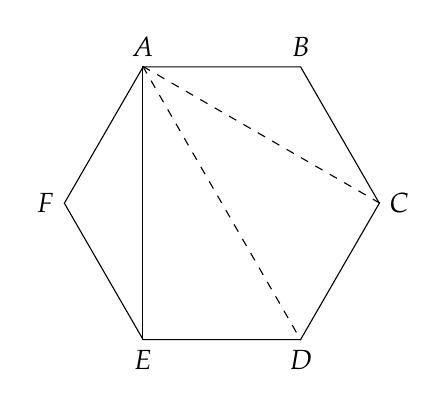
\begin{tikzpicture}
\node[name=hexagon, regular polygon, regular polygon sides=6, minimum size=4cm, draw] at (0,0) {};
\draw (hexagon.corner 2) -- (hexagon.corner 4);
\draw [dashed] (hexagon.corner 2) -- (hexagon.corner 5);
\draw [dashed] (hexagon.corner 2) -- (hexagon.corner 6);
\foreach \anchor/\placement/\name in {corner 1/above/$B$, corner 2/above/$A$, corner 3/left/$F$, corner 4/below/$E$, corner 5/below/$D$, corner 6/right/$C$}
\draw (hexagon.\anchor) node[\placement] {\name};
\end{tikzpicture}
\caption{Non-intersecting diagonals}\label{fig.diag}
\end{center}
\end{figure}

\begin{exercise}\label{e.diag}
For a convex polygon with $n$ sides, the number of (possibly intersecting) diagonals is $\frac{1}{2}n(n-3)$.
\end{exercise}

\begin{exercise}
For a convex polygon with $n$ sides, the sum of the interior angles is $180(n-2)^{\circ}$.
\end{exercise}

\begin{exercise}
Given a line of length $1$ and a number $n\geq 1$, construct a line of length $\sqrt n$.
\end{exercise}
Hint: Pythagoras's theorem.

\section{Trees}

A binary tree is a graph with nodes and edges, such that there is one node at the top, the \emph{root}, and each node is connect to by edges to zero, one or two other nodes called its descendants. A node with no descendants is a \emph{leaf} and a node which is not a leaf is an \emph{internal node}. The height of the tree is the length of the longest path from the root to a leaf.

A binary tree all of whose leaves are at the same height $h$ and all of whose internal nodes have exactly two descendants is called a \emph{complete binary tree} (Figure~\ref{fig.complete}). 

\begin{figure}[b]
\begin{center}
\begin{tikzpicture}%
[dots/.style={fill, inner sep=0pt, minimum size=3pt, shape=circle},%
level 1/.style={sibling distance=2cm},%
level 2/.style={sibling distance=1.5cm}]

\node[dots] at (7.5,0) {}
child {
  node[dots] {} coordinate (L1)
  child { node[dots] {} coordinate (L2)}
  child { node[dots] {}}
}
child {
  node[dots] {}
  child { node[dots] {}}
  child { node[dots] {}}
};

\node[dots] at (3,0 |- L1) {}
child { node[dots] {}}
child { node[dots] {}};

\node[dots] at (0,0 |- L2) {};

\node at (0,-3.5) {(a)};
\node at (3,-3.5) {(b)};
\node at (7.5,-3.5) {(c)};
\end{tikzpicture}
\caption{Complete binary trees of heights $1$, $2$, $3$}\label{fig.complete}
\end{center}
\end{figure}

\begin{theorem}
Let $n_h$ be the number of nodes in a complete binary tree of
height $h$. Then $n_h = 2^{h+1}-1$.
\end{theorem}

\textbf{Example} In Figure~\ref{fig.complete}: (a) $n_0=2^1-1=1$,$\,$ (b) $n_1 = 2^2-1=3$,$\,$ (c) $n_2 = 2^3-1=7$.

\textbf{Proof} The base case is a leaf which is a tree of height $0$: $1 = 2^{0+1}-1=1$. The inductive hypothesis that the number of nodes in the left subtree ($n_l$) and the number of nodes in the right subtree ($n_r$), both of height $h$, are given by the formula $n_l=n_r=2^{h+1}-1$. To prove the inductive step, note that a tree of height $h+1$ is constructed from two subtrees of height $h$ together with \emph{one} additional node which is the new root. Therefore:
\[
n_{h+1} = n_l + n_r + 1 \ih{} (2^{h+1}-1) + (2^{h+1}-1) + 1 = 2\cdot 2^{h+1} -2 +1= 2^{(h+1)+1} - 1\,.
\]

\qedd{5}

Although the induction is mathematical induction on the height of the tree, the tree itself is constructed inductively from two subtrees. In the following exercise, this will become more apparent.

\begin{exercise}
Let $n_h$ be the number of nodes in an (arbitrary) binary tree of height $h$. Then $n_h\leq 2^{h+1}-1$.
\end{exercise}

\textbf{Example} Figure~\ref{fig.incomplete} a binary tree of height $2$ with $5 \leq 2^3-1=7$ nodes.

\begin{figure}[t]
\begin{center}
\begin{tikzpicture}%
[dots/.style={fill, inner sep=0pt, minimum size=3pt, shape=circle},%
level 1/.style={sibling distance=2cm},%
level 2/.style={sibling distance=1.5cm}]
\node[dots] at (0,0) {}
child {
  node[dots] {}
  child { node[dots] {}}
  child { node[dots] {}}
}
child {
  node[dots] {}
};
\end{tikzpicture}
\caption{Incomplete binary tree of height $2$ with $5$ nodes}\label{fig.incomplete}
\end{center}
\end{figure}

\section{Graphs}

A \emph{graph} is an arbitrary structure consisting of nodes and edges. If a set of edges form a \emph{cycle}, then they enclose a \emph{surface}. We also count the area not enclosed in any cycle as a surface. %Figure~\ref{fig.euler}
The following figure shows a graph with $7$ nodes, $8$ edges and $3$ surfaces, where surface $s_3$ is labeled several times to emphasize that it includes all the plane not enclosed in the two cycles:

%\begin{figure}[hbt]
\begin{center}
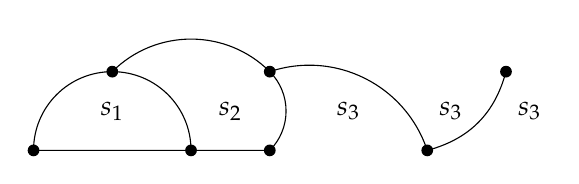
\begin{tikzpicture}
\draw (0,0) to [bend left=45] (1,1) to [bend left=45] (3,1) to [bend left=45] (3,0) to cycle;
\draw (1,1) to [bend left=45] (2,0);
\draw (3,1) to [bend left=45] (5,0) to [bend right=30] (6,1);
\foreach \x in {(0,0),(1,1),(2,0),(3,0),(3,1),(5,0),(6,1)}
  \node[shape=circle,fill,inner sep=1.5pt] at \x {};
\foreach \x/\i in {1/$s_1$,2.5/$s_2$,4/$s_3$,5.3/$s_3$,6.3/$s_3$}
  \node at (\x,0.5) {\i};
\end{tikzpicture}
%\caption{A graph with $7$ nodes, $8$ edges and $3$ surfaces}\label{fig.euler}
\end{center}
%\end{figure}

\begin{exercise} (\textbf{Euler})
For a graph with $n$ nodes, $e$ edges and $s$ surfaces, $s+n=e+2$.
\end{exercise}
\textbf{Example} In the figure, $3+7=8+2$.

Hint: Prove by induction on the number of edges in the graphs. There are two inductive steps depending on whether an edge is part of a cycle or not.

%%%%%%%%%%%%%%%%%%%%%%%%%%%%%%%%%%%%%%%%%%%%%%%%%%%%%%%%%%%%%%%%%%%

\chapter{Things to Watch Out For}\label{s.watch}

Let us point out several issues concerning induction that you should watch out for.

\section{Induction is not the only method of proof}

While induction is widely used and in many cases it is the only way or the best way of proving a theorem, it is not the only method of proof. Here is a proof of Theorem~\ref{t.div2} that does not use induction.

\textbf{Theorem} For $n\geq 1$, $n(n+1)$ is divisible by $2$.

\textbf{Proof} If $n$ is divisible by $2$ we are done. Otherwise, $n=2k+1$ for some $k$. Then $n+1=2k+2=2(k+1)$ is divisible by $2$.\qed

This is really the same as the inductive step of the inductive proof.

\begin{exercise} Prove without using induction: For $n\geq 1$, $n(n+1)(n+2)$ is divisible by $3$.
\end{exercise}

Carl Friedrich Gauss was one of the most important mathematicians. According to an apocryphal story, when he acted up in elementary school, his teacher forced him to compute the sum of the first $100$ integers in the hope that it would keep him quiet for quite some time. Gauss noted that the numbers could be arranged as follows:
\[
\begin{array}{crrrrrrr}
& 1 & 2 & 3 & \cdots & 98 & 99 & 100\\
+& 100 & 99 & 98 & \cdots & 3 & 2 & 1\\
\hline
& 101 & 101 & 101 & \cdots & 101 & 101 & 101\\
\end{array}
\]
which leads immediately to the formula $\frac{100\cdot 101}{2}$ that we proved in Theorem~\ref{t.sum}. 

A non-inductive proof for arbitrary $n$ is:
\begin{eqnarray*}
\sum_{i=1}^{n} i &=& \sum_{i=1}^{n} (n-i+1)\\
&=& \frac{1}{2}\left[\sum_{i=1}^{n} i + \sum_{i=1}^{n} (n-i+1)\right]\\
&=& \frac{1}{2}\left[\sum_{i=1}^{n} (n+1)\right]\\
&=& \frac{n(n+1)}{2}\,.
\end{eqnarray*}

\begin{exercise}
Prove with and without induction that $x-1$ divides $x^n-1$. Which proof do you prefer?
\end{exercise}

Hint: For the non-inductive proof, compute $(x-1)\sum_{i=0}^{i=n}x^i$. For the inductive proof find polynomials $p(x),q(x)$, both divisible by $x-1$, such that $x^{n+1} - 1 =p(x)+q(x)$.

\section{Sometimes you can't use induction}

Induction can only be used if larger structures are constructed in a discrete, step-by-step manner from smaller structures, and if there is a simplest structure. Properties of the rational numbers similar to the ones we have proved for the integers cannot be proved using mathematical induction because there is no ``first'' rational number and there is no ``next'' rational number.\footnote{Georg Cantor found a way of enumerating the positive rational numbers $\{\frac{1}{1},\frac{1}{2},\frac{2}{1},\frac{1}{3},\frac{3}{1},\frac{1}{4},\frac{2}{3},\frac{3}{2},\frac{4}{1},\frac{1}{5},\frac{5}{1},\ldots\}$, but this sequence is not intuitive and is not appropriate for inductive proofs.} Suppose that we want to prove that for any \emph{positive} rational numbers $a,b$ such that $a<b$, $a\leq \frac{a+b}{2} \leq b$.

\begin{itemize}
\item What is the base case? Suppose $a$ is the \emph{smallest} positive rational number; then $\frac{a}{2}$ is positive, rational and \emph{less than} $a$.
\item What is the inductive hypothesis and how is the inductive step proved? Suppose the inductive hypothesis is that a formula is true for $a,b$. In the inductive step, we need to prove it for the \emph{next} pair of values, which can be written as $a+\frac{p_a}{q_a}$, $b+\frac{p_b}{q_b}$. But $a+\frac{p_a}{q_a+1}$, is greater than $a$ and less than $a+\frac{p_a}{q_a}$, so there is no next pair of values.
\end{itemize}

\section{Watch out for incorrect proofs}

\begin{theorem}
For $n\geq 0$ and $a\geq 1$, $a^n=1$.
\end{theorem}

\textbf{Proof} Base case: $a^0=1$. Inductive hypothesis: $a^k=1$ for $0\leq k\leq n$. The inductive step is:
\[
a^{n+1}=a^n\cdot a \ih{} 1\cdot a = a = \frac{a^{n-1}}{a^{n-2}} \ih{} \frac{a^{n-1}}{1} \ih{} \frac{1}{1} = 1.
\]

\qedd{4}

\smallskip

Of course, this is nonsense because $2^3=8 \neq 1$.

\begin{exercise}
Where is the error in this proof?
\end{exercise}

\begin{theorem}
All the students in a set (a classroom) have the same hair color.
\end{theorem}

\textbf{Proof} Base case: Pick any student $s_1$. He or she has hair colored $c$. Inductive hypothesis: In any set of $n$ students, all students have the same color hair $c$. Inductive step: Let $s_1,s_2,\ldots,s_n,s_{n+1}$ be the students in a set with $n+1$ students. Consider the subset of students $s_1,s_2,\ldots,s_n$; by the inductive hypothesis they have the same hair color $c$. Similarly, consider the subset of students $s_1,s_2,\ldots,s_{n-1},s_{n+1}$; by the inductive hypothesis they have the same hair color $c$. So the color of $s_{n+1}$'s hair is $c$, the same as that of $s_1$, which is the same as that of $s_2,\ldots,s_n$. Therefore, all of $s_1,s_2,\ldots,s_n,s_{n+1}$ have hair colored $c$.\qed

Different students have different hair colors (to say nothing of those who dye their hair in all sorts of novel colors!), so clearly this proof is incorrect.

\begin{exercise}
Where is the error in this proof?
\end{exercise}

%%%%%%%%%%%%%%%%%%%%%%%%%%%%%%%%%%%%%%%%%%%%%%%%%%%%%%%%%%%%%%%%%%%

\chapter{Mathematical Logic}\label{s.logic}

Induction is an essential tool in mathematical logic because theorems are statements of properties of \emph{all} formulas. Since formulas are constructed by combining subformulas using logical operators, the induction is on the structure of a formula. In this section, we show how induction is used, often implicitly, in proofs in propositional logic.

\begin{definition}
A formula $A$ is \emph{satisfiable} if and only if there is an assignment of $T$ or $F$ to each atomic proposition such that $A$ evaluates to $T$.
\end{definition}

\begin{definition}
Formula $A$ is \emph{logically equivalent} to formula $A'$ if and only if they evaluate to the same value for every assignment to their atomic propositions. Notation: $A\equiv A'$.
\end{definition}

Here is an example to clarify the difference between the concepts of logical equivalence and satisfiable if and only if satisfiable. Consider the two formulas:
\[
\begin{array}{l}
A=(p \vee q \vee \neg r) \;\wedge\; (p \vee \neg q) \;\wedge\; (\neg p \vee q)\,,\\
B=(p \vee \neg q) \;\wedge\; (\neg p \vee q)\,.
\end{array}
\]
$A$ is satisfiable because it evaluates to $T$ under the assignment $\{p=F,q=F,r=F\}$ and $B$ is satisfiable under the same assignment. However, under the assignment $\{p=F,q=F,r=T\}$, $A$ evaluates to $F$ and $B$ evaluates to $T$, so they are not logically equivalent.

\section{Transforming a formula into CNF}

\begin{definition}
A formula of propositional logic is in \emph{conjunctive normal form (CNF)} if it is a conjunction (and) of disjunctions (or) of literals (atomic propositions or their negations).
\end{definition}

\vspace*{-10pt}
\textbf{Example} The following formula is not in CNF:
\begin{equation}\label{eq.logic}
(p \wedge \neg q) \;\rightarrow\; (\neg q \wedge p)\,,
\end{equation}
but it is logically equivalent to the following formula in CNF:
\begin{equation}\label{eq.cnf3}
(\neg p \vee q \vee \neg q) \;\wedge\; (\neg p \vee q \vee p)\,.
\end{equation}

CNF is extremely important in computer science, both in theory and in practice. Stephen Cook proved the fundamental theoretical result that determining the satisfiability of CNF formulas is NP-complete. Logic is used in proving theorems by resolution, in logic programming and for SAT solving.

\begin{theorem}\label{t.cnf}
Given a formula $A$ in propositional logic, a CNF formula $A'$ can be constructed such that $A\equiv A'$.
\end{theorem}

We won't give a full proof here; instead, we demonstrate it on Formula~\ref{eq.logic}:

\begin{center}
\begin{tabular}{l@{\hspace{2em}}l}
$(p \wedge \neg q) \;\rightarrow\; (\neg q \wedge p)$&Original formula\\
$\neg (p \wedge \neg q) \;\vee\; (\neg q \wedge p)$&Eliminate $\rightarrow$\\
$(\neg p \vee \neg \neg q) \;\vee\; (\neg q \wedge p)$&Push negation inwards\\
$(\neg p \vee q) \;\vee\; (\neg q \wedge p)$&Eliminate $\neg\neg$\\
$(\neg p \vee q \vee \neg q) \;\wedge\; (\neg p \vee q \vee p)$&Distributive law\\
\end{tabular}
\end{center}
The justifications are based upon logical equivalences that can be proved:
\begin{eqnarray*}
(A\rightarrow B) &\equiv& (\neg A \vee B)\\
\neg (A \vee B) &\equiv& (\neg A \wedge \neg B)\\
\neg (A \wedge B) &\equiv& (\neg A \vee \neg B)\\
\neg\neg A &\equiv& A\\
(A\vee (B\wedge C)) &\equiv& ((A \vee B) \wedge (A \vee C))\,.
\end{eqnarray*}
The proof of Theorem~\ref{t.cnf} is a sequence of lemmas such as:
\begin{lemma}
Let $A$ be a formula. Then there is a formula $A'$ without the operator $\rightarrow$ such that $A\equiv A'$.
\end{lemma}
This seems innocent enough once we have proved that $(A\rightarrow B) \equiv (\neg A \vee B)$, but it is hiding an implicit induction.

\textbf{Proof} The base case is where $A$ is $p$, an atomic proposition, but $p$ does not contain the operator $\rightarrow$ so the claim is trivial. The inductive hypothesis is that for any formula $A$ of size\footnote{The size of a formula can be defined in terms of the height of the formation tree of the formula, but the details are beyond the scope of this work.}
 less than or equal to $n$, there is an equivalent formula $A'$ without $\rightarrow$. Let $A_1 \vee A_2$ be a formula such that the sizes of $A_1, A_2$ are less than or equal to $n$. By the inductive hypothesis, there are formulas $A_1', A_2'$ without $\rightarrow$, such that $A_1\equiv A_1'$ and $A_2\equiv A_2'$. Clearly, $A_1' \vee A_2' = A'$ is equivalent to $A$ and does not use $\rightarrow$.

Similar inductive steps hold for $\neg A_1$ and $A_1 \wedge A_2$.

For $A_1 \rightarrow A_2$, by the inductive hypothesis, there are formulas $A_1', A_2'$ without $\rightarrow$, such that $A_1\equiv A_1'$ and $A_2\equiv A_2'$. Then $A_1 \rightarrow A_2 \equiv \neg A_1 \vee A_2 \equiv \neg A_1' \vee A_2' = A'$, a formula that does not use $\rightarrow$.\qed

To finish the proof of Theorem~\ref{t.cnf} we need another three lemmas of similar complexity. Each inductive proof is on the \emph{structure} of the formula with the number of inductive steps equal to the number of operators in the logic.\footnote{At least four operators ($\neg,\vee,\wedge,\rightarrow$) and sometimes four other operators ($\leftrightarrow$ (equivalent), $\oplus$ (xor), $\uparrow$ (nand) and $\downarrow$ (nor)) are used. Raymond Smullyan introduced a simplified notation of $\alpha$ (conjunctive) and $\beta$ (disjunctive) operators, so that there are only two inductive steps in proofs.} No textbook in mathematical logic would write the proof in such great detail, because the result is clear from equivalences like $(A\rightarrow B)\equiv(\neg A \vee B)$, but it important to realize that induction is being used implicitly.

\section{The reduction from CNF to 3CNF}

\begin{definition}
A formula in CNF is in \emph{3CNF} if and only if each disjunction has exactly three literals in each disjunction.
\end{definition}

\vspace*{-10pt}

\textbf{Example} Formula~\ref{eq.cnf3} is in 3CNF.

\begin{theorem}\label{t.cnf3}
Given a formula $A$ in propositional logic, a 3CNF formula $A'$ can be constructed such that $A$ is satisfiable if and only if $A'$ is satisfiable.
\end{theorem}

\vspace*{-10pt}

Theorem~\ref{t.cnf3} shows that the satisfiability of 3CNF formulas is NP-complete.

The usual proof of Theorem~\ref{t.cnf3} uses induction implicitly; here we give a proof that makes the induction explicit.

\textbf{Proof} It is sufficient to show that any single disjunction $A=x_1 \vee x_2 \vee \cdots \vee x_n$ can be transformed into a conjunction of disjunctions with three literals each.

There are three base cases:
\begin{itemize}
\item If $A$ has three literals, there is nothing to do.

\item If $A$ has two literals $p_1\vee p_2$, let $A'$ be:
\[
(p_1 \vee p_2 \vee q) \;\wedge\; (p_1 \vee p_2 \vee \neg q)\,,
\]
where $q$ is a new atomic proposition. If $A$ is satisfiable then either $p_1$ or $p_2$ is assigned $T$, and $A'$ also evaluates to $T$. Conversely, suppose that $A'$ is satisfiable. But neither of the assignments $\{p_1=F,p_2=F,q=T\}$ and $\{p_1=F,p_2=F,q=F\}$ satisfy $A'$, so either $p_1$ or $p_2$ (or both) must be assigned $T$. It follows that $A$ is also satisfiable.

\item
\begin{exercise}
If $A$ is a single literal $p$ or $\neg p$, there is a formula $A'$ with exactly three literals that is satisfiable if and only if $A$ is satisfiable. 
\end{exercise}
Hint: How many new atomic propositions must be used?
\end{itemize}

The inductive hypothesis is: If $A=p_1 \vee p_2 \vee \cdots \vee p_n$ is a disjunction with $n\geq 3$ literals, there exists a 3CNF formula $A'$ which is satisfiable if and only if $A$ is statisfiable. The inductive step is: Let $A$ be a disjunction $p_1 \vee p_2 \vee \cdots \vee p_n \vee p_{n+1}$ with $n+1$ literals and construct $A'$ as:
\begin{displaymath}
(p_1 \vee \cdots \vee p_{n-1} \vee q) \;\wedge\; (\neg q \vee p_n \vee p_{n+1})\,,
\end{displaymath}
where $q$ is a new atomic proposition. We can show that $A'$ is satisfiable if and only if $A$ is satisfiable using a proof similar to that for the base case of two literals.

Now apply the inductive hypothesis to the first disjunction with $n$ literals to obtain a formula $A''$ in 3CNF that is satisfiable if and only if the disjunction is satisfiable. Then:
\begin{displaymath}
A'' \;\wedge\; (\neg q \vee p_n \vee p_{n+1})
\end{displaymath}
is a 3CNF formula that is satisfiable if and only if $A$ is satisfiable.\qed

%%%%%%%%%%%%%%%%%%%%%%%%%%%%%%%%%%%%%%%%%%%%%%%%%%%%%%%%%%%%%%%%%%%

\chapter{Models of Computation}\label{s.models}

Models of computation, such as automata and formal languages, are a fundamental topic of theoretical computer science. Proofs use induction over the structure of an automaton or the derivation of a string from a formal grammar. There may often be more than one base case and more than one inductive step.

We assume that the reader is familiar with the concepts of nondeterministic finite automata (NFA) and regular expressions (RE).

\section{Automata}

\begin{theorem}
Let $r$ be an RE. Then an NFA can be constructed that accepts the language of $r$.
\end{theorem}

\textbf{Proof} There are \emph{three} base cases:
\begin{itemize}
\item $r$ is the empty set $\emptyset$. The NFA consisting of one initial and one final state with no transitions accepts no strings at all.
\begin{center}
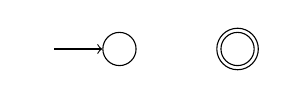
\begin{tikzpicture}[circle]
\node (dummy) at (-1,0) {};
\node (initial) at (0,0) [draw,minimum size=12pt] {};
\node (final) at (1.5,0) [draw,minimum size=15pt] {};
\node at (1.5,0) [draw,minimum size=12pt] {};
\draw[->] (dummy) -- (initial);
\end{tikzpicture}
\end{center}
\item $r$ is the null string $\epsilon$. The NFA consisting of one state which is both initial and final accepts the null string:
\begin{center}
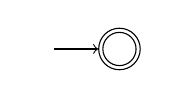
\begin{tikzpicture}[circle]
\node (dummy) at (-1,0) {};
\node (final) at (0,0) [draw,minimum size=15pt] {};
\node at (0,0) [draw,minimum size=12pt] {};
\draw[->] (dummy) -- (final);
\end{tikzpicture}
\end{center}
\item $r$ is a single symbol $a$. The following NFA accepts the language $\{a\}$:
\begin{center}
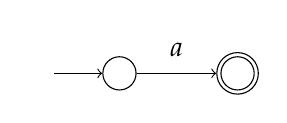
\begin{tikzpicture}[circle]
\node (dummy) at (-1,0) {};
\node (initial) at (0,0) [draw,minimum size=12pt] {};
\node (final) at (1.5,0) [draw,minimum size=15pt] {};
\node at (1.5,0) [draw,minimum size=12pt] {};
\draw[->] (dummy) -- (initial);
\draw[->] (initial) -- node[above] {$a$} (final);
\end{tikzpicture}
\end{center}
\end{itemize}

There are \emph{three} inductive steps, one for each of the three ways of constructing an RE from simpler REs:

\begin{itemize}
\item Concatenation $r_1r_2$: By the inductive hypothesis there are NFAs $\mathit{nfa}_1$ and $\mathit{nfa}_2$ that accept the languages of $r_1$ and $r_2$, respectively. Construct $\mathit{nfa}_{12}$ by adding a null transition from the final state of $\mathit{nfa}_1$ to the initial state of $\mathit{nfa}_2$. The initial state of $\mathit{nfa}_{12}$ is the initial state of $\mathit{nfa}_1$ and its final state is the final state of $\mathit{nfa}_2$.
\begin{center}
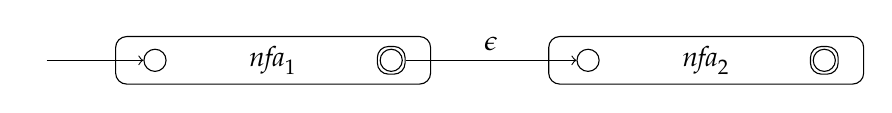
\begin{tikzpicture}[rounded corners]
\node (dummy) at (-3,0) {};
\node at (0,0) [draw,rectangle,minimum width=4cm,minimum height=.5cm] {$\mathit{nfa}_1$};
\node (initial) at (-1.5,0) [draw,minimum size=8] {};
\node (final1) at (1.5,0) [draw,minimum size=10pt] {};
\node at (1.5,0) [draw,minimum size=8] {};
\node at (5.5,0) [draw,rectangle,minimum width=4cm,minimum height=.5cm] {$\mathit{nfa}_2$};
\node (initial2) at (4,0) [draw,minimum size=8] {};
\node at (7,0) [draw,minimum size=10pt] {};
\node at (7,0) [draw,minimum size=8] {};
\draw[->] (dummy) -- (initial);
\draw[->] (final1) -- node[above] {$\epsilon$} (initial2);
\end{tikzpicture}
\end{center}

\item Union $r_1+r_2$: By the inductive hypothesis there are NFAs $\mathit{nfa}_1$ and $\mathit{nfa}_2$ that accept the languages of $r_1$ and $r_2$, respectively. Construct $\mathit{nfa}_{12}$ by adding new start and final states and null transitions.
\begin{center}
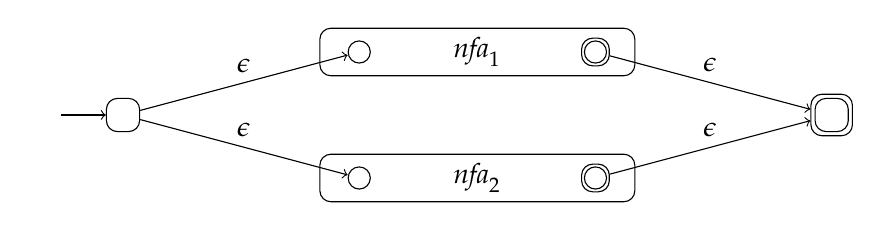
\begin{tikzpicture}[minimum size=12pt,rounded corners]
\node (initial) at (-2,0) [draw] {};
\node (final) at (7,0) [draw,minimum size=15pt] {};
\node at (7,0) [draw] {};
\node (dummy) at (-3,0) {};
\node at (2.5,.8) [draw,rectangle,minimum width=4cm,minimum height=.5cm] {$\mathit{nfa}_1$};
\node at (2.5,-.8) [draw,rectangle,minimum width=4cm,minimum height=.5cm] {$\mathit{nfa}_2$};
\node (top-initial) at (1,.8) [draw,minimum size=8] {};
\node (top-final) at (4,.8) [draw,minimum size=10pt] {};
\node at (4,.8) [draw,minimum size=8] {};
\node (bottom-initial) at (1,-.8) [draw,minimum size=8] {};
\node (bottom-final) at (4,-.8) [draw,minimum size=10pt] {};
\node at (4,-.8) [draw,minimum size=8] {};
\draw[->] (dummy) -- (initial);
\draw[->] (initial) -- node[above] {$\epsilon$} (top-initial);
\draw[->] (initial) -- node[above] {$\epsilon$} (bottom-initial);
\draw[->] (top-final) -- node[above] {$\epsilon$} (final);
\draw[->] (bottom-final) -- node[above] {$\epsilon$} (final);
\end{tikzpicture}
\end{center}

\item Closure $r^*$: By the inductive hypothesis there is an NFA $\mathit{nfa}_r$ that accepts the language of $r$. Add new initial and final states and null transitions as shown in the diagram:
\begin{center}
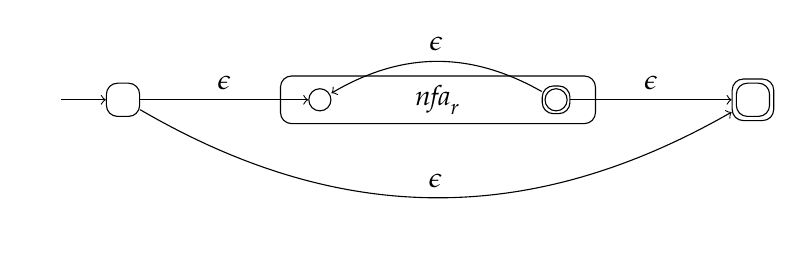
\begin{tikzpicture}[minimum size=12pt,rounded corners]
\node (initial) at (0,0) [draw] {};
\node (final) at (8,0) [draw,minimum size=15pt] {};
\node at (8,0) [draw] {};
\node (initial1) at (2.5,0) [draw,minimum size=8] {};
\node (final1) at (5.5,0) [draw,minimum size=10pt] {};
\node at (5.5,0) [draw,minimum size=8] {};
\draw[->] (final1) to [bend right=30] node[above] {$\epsilon$} (initial1);
\node (dummy) at (-1,0) {};
\node at (4,0) [draw,rectangle,minimum width=4cm,minimum height=.5cm] {$\mathit{nfa}_r$};
\draw[->] (dummy) -- (initial);
\draw[->] (initial) -- node[above] {$\epsilon$} (initial1);
\draw[->] (final1) -- node[above] {$\epsilon$} (final);
\draw[->] (initial) to [bend right=30] node[above] {$\epsilon$} (final);
\end{tikzpicture}
\end{center}
The null transition from the initial state to the final state is taken for strings generated by zero instances of $r$, and the internal transition from the final state of $\mathit{nfa}_r$ to its initial state is for one or more repetitions of $r$.
\end{itemize}
\qedd{5}

\section{Formal languages}

Proofs in formal language theory use induction over the length of the generated strings, which is really induction over the generation of the string from a grammar. Consider the context-free grammar $G$:

\begin{displaymath}
\begin{array}{l@{\hspace{2em}}l@{\hspace{2em}}l@{\hspace{2em}}l}
S \rightarrow aB & S \rightarrow bA & A \rightarrow a & B \rightarrow b \\
A \rightarrow aS & B \rightarrow bS & A \rightarrow bAA & B \rightarrow aBB\\
\end{array}
\end{displaymath}

\begin{theorem}
The language $L$ generated by the grammar $G$
is the set of all words over $\{a,b\}$ with an equal number of $a$'s and
$b$'s, symbolically:

\begin{displaymath}
S \stackrel{*}{\Rightarrow} w \;\;\mathrm{iff}\;\; \#a = \#b,
\end{displaymath}
where $\#a,\#b$ are the number of $a$'s and $b$'s in $w$.
\end{theorem}

\textbf{Proof} We will use induction \emph{simultaneously} to prove the following three claims:
\begin{eqnarray}
S \stackrel{*}{\Rightarrow} w &\;\;\mathrm{iff}\;\;& \#a = \#b\label{eq.formal1}\\
A \stackrel{*}{\Rightarrow} w &\;\;\mathrm{iff}\;\;& \#a = \#b+1\label{eq.formal2}\\
B \stackrel{*}{\Rightarrow} w &\;\;\mathrm{iff}\;\;& \#a+1 = \#b.\label{eq.formal3}
\end{eqnarray}
The base case $|w|=1$ is trivial because $A$ and $B$ generate
$a$ and $b$, respectively, and $S$ generates no strings of length one,
although we do have to note that these are the \emph{only} ways that a
string of length one can be generated.

Let $w$ be a word derived from $S$ with $|w|=n+1$. There are three inductive steps and to prove each we assume \emph{all} three claims for $|w|=n$ as inductive hypotheses. 

We start by proving Formula~\ref{eq.formal1} for $w$. The first step in the derivation is $S\rightarrow aB \stackrel{*}{\Rightarrow} aw'$ or $S\rightarrow bA\stackrel{*}{\Rightarrow} bw'$. In the first case, by the inductive hypothesis in Formula~\ref{eq.formal3}, the word $w'$ (generated by $B$) has $\#a+1=\#b$, so $\#a=\#b$ in $w$. A similar proof holds for the second case using Formula~\ref{eq.formal2}.

The rest of the proof is left as an exercise.\qed

\begin{exercise}\mbox{}
\begin{itemize}
\item Prove Formulas~\ref{eq.formal2} and~\ref{eq.formal3}.
\item Prove the converse: If $\#a=\#b$ in $w$ then $S \stackrel{*}{\Rightarrow} w$.
\end{itemize}
\end{exercise}

%%%%%%%%%%%%%%%%%%%%%%%%%%%%%%%%%%%%%%%%%%%%%%%%%%%%%%%%%%%%%%%%%%%

\chapter{Program Verification}\label{s.verif}

A computer program is not \emph{correct} if some computation does not fulfill its specification. For example, if a program is specified to compute the square root of a number but instead computes its cube root, the program is not correct, although it would be if the specification had asked for the cube root. There are techniques for formally specifying computer programs and their computations, and for \emph{proving} that a program is correct.

The \emph{length of a computation} of a program can be indefinitely long. Furthermore, the \emph{number of computations} of a program can be unbounded: there will be a different computation for each value of a numeric input. We naturally turn to induction in order to prove properties of a potentially infinite structure and an unlimited number of structures.

We demonstrate inductive proofs using both sequential and concurrent programs. A sequential program is usually \emph{functional}: it receives an input and then computes an output in a finite number of steps. The example we consider is an algorithm to sort a sequence of numbers: the input is the original sequence and the output is a sequence with the numbers ordered by value. We use induction to prove correctness of the algorithm no matter how many numbers there are in the sequence.

Concurrent programs consist of several sequential programs (called \emph{processes}) running at the same time. Concurrent programs are usually \emph{reactive}, not functional: they are expected to run forever, reacting to an input that may be received at an arbitrary point in time and producing an output very shortly after receiving the input. For example, the operating system on your smartphone is always running; when you touch an icon, there is a visible reaction. Here induction is essential: not only is the length of the computation infinite, but there are an infinite number of ways of \emph{interleaving} the computations of the processes forming the concurrent program.

\section{Sequential programs}

Consider a array of integers such as:\footnote{The term \emph{array} is used in computer science for what mathematicians call a \emph{vector}.}
\[
A=[5,31,7,1,6,17,16,22,3,10]\,.
\]
We want an algorithm to \emph{sort} the array $A$: construct an array $B$ whose elements are a permutation of the elements of $A$ in ascending order:
\[
B=[1,3,5,6,7,10,16,17,22,31]\,.
\]
Here we consider two simple algorithms that are relatively efficient.

\textbf{\Large Insertion sort}

When playing cards, it is polite to wait until all the cards in the hand have been dealt and only then to gather them up and arrange them. If you are not polite, you can use an efficient algorithm called \emph{insertion sort}: Pick the cards up one-by-one and place each one in its proper position.\footnote{We omit the statements for the case where the new element is the smallest one in $A$.} 
\begin{verbatim}
    while A is not empty
      move the first element of A after
          the largest element in B with a smaller value
\end{verbatim}
For the example above, the array $B$ would be built as follows:
\[
\begin{array}{lll}
B_0&=&[\,]\\
B_1&=&[5]\\
B_2&=&[5,31]\\
B_3&=&[5,7,31]\\
B_4&=&[1,5,7,31]\\
B_5&=&[1,5,6,7,31]\\
B_6&=&[1,5,6,7,17,31]\\
B_7&=&[1,5,6,7,16,17,31]\\
B_8&=&[1,5,6,7,16,17,22,31]\\
B_9&=&[1,3,5,6,7,16,17,22,31]\\
B_{10}&=&[1,3,5,6,7,10,16,17,22,31]\\
\end{array}
\begin{array}{lll}
A_0&=&[5,31,7,1,6,17,16,22,3,10]\\
A_1&=&[31,7,1,6,17,16,22,3,10]\\
A_2&=&[7,1,6,17,16,22,3,10]\\
A_3&=&[1,6,17,16,22,3,10]\\
A_4&=&[6,17,16,22,3,10]\\
A_5&=&[17,16,22,3,10]\\
A_6&=&[16,22,3,10]\\
A_7&=&[22,3,10]\\
A_8&=&[3,10]\\
A_9&=&[10]\\
A_{10}&=&[\,]\\
\end{array}
\]
Let us prove the correctness of insertion sort for an array $A$ of arbitrary length $n$.

\textbf{Correctness claim:} When the insertion sort algorithm terminates, the elements of $B$ are an ordered permutation of the elements of $A$.

\textbf{Lemma 1:} For all $i$, the sequence composed of the elements in $B_i$ followed by the elements of $A_i$ is a permutation of $A$.

\textbf{Lemma 2:} For all $i$, the sequence of elements in $B_i$ is ordered.

The correctness claim follows immediately from the lemmas: when the computation terminates, $A_n$ is empty, so by Lemma 1, $B_n$ itself is a permutation of the elements of $A$, and by Lemma 2 $B_n$ is ordered.

We omit the trivial proof of Lemma 1.

\textbf{Proof of Lemma 2:} Base case: $B_0$ is empty so it is vacuously ordered. Inductive step: Assume that $B_i$ is ordered and suppose that $a_i$ is the first element of $A_i$ and that $b_k$ is the largest element of $B_i$ such that $b_k < a_i \leq b_{k+1}$. Then $B_{i+1} = [\ldots,b_k,a_i,b_{k+1},\ldots]$ is ordered.

\bigskip

\textbf{\Large Selection sort}

Selection sort is easier to implement than insertion sort and is also efficient:
\begin{verbatim}
    while A is not empty
      move the smallest element of A to the end of B
\end{verbatim}
For the example, the arrays are:
\[
\begin{array}{lll}
B_0&=&[\,]\\
B_1&=&[1]\\
B_2&=&[1,3]\\
B_3&=&[1,3,5]\\
B_4&=&[1,3,5,6]\\
B_5&=&[1,3,5,6,7]\\
B_6&=&[1,3,5,6,7,10]\\
B_7&=&[1,3,5,6,7,10,16]\\
B_8&=&[1,3,5,6,7,10,16,17]\\
B_9&=&[1,3,5,6,7,10,16,17,22]\\
B_{10}&=&[1,3,5,6,7,10,16,17,22,31]\\
\end{array}
\begin{array}{lll}
A_0&=&[5,31,7,1,6,17,16,22,3,10]\\
A_1&=&[5,31,7,6,17,16,22,3,10]\\
A_2&=&[5,31,7,6,17,16,22,10]\\
A_3&=&[31,7,6,17,16,22,10]\\
A_4&=&[31,7,17,16,22,10]\\
A_5&=&[31,17,16,22,10]\\
A_6&=&[31,17,16,22]\\
A_7&=&[31,17,22]\\
A_8&=&[31,22]\\
A_9&=&[31]\\
A_{10}&=&[\,]\\
\end{array}
\]
To prove the correctness of selection sort, we need two lemmas: the first is the trivial Lemma 1 given above for insertion sort.

\begin{exercise}
State and prove the lemma needed to prove the correctness of selection sort.
\end{exercise}


\section{Concurrent programs}

Concurrent programs are notorious for their elusive \emph{race conditions}: the relative speeds of execution of the processes forming the program can cause obscure errors which are extremely difficult to find and to replicate for testing. \emph{Semaphores} are a simple but effective synchronization mechanism that can be used to prevent race conditions. We assume that you are familiar with the definition of semaphores and their operations, and with the trivial program for achieving mutual exclusion using semaphores:

\begin{verbatim}
                        global int sem = 1
        process p                          process q
        loop forever                       loop forever
            p1: wait(sem)                      q1: wait(sem)
            p2: critical section               q2: critical section
            p3: signal(sem)                    q3: signal(sem)
\end{verbatim}

The following formulas are invariant---true in every state of every computation:
\begin{eqnarray}
(\mathit{sem} = 0) \vee (\mathit{sem} = 1)&&\label{eq.sem01}\\
\#\mathit{CS} + \mathit{sem} = 1,&&\label{eq.sem}
\end{eqnarray}
where $\mathit{sem}$ is the value of the variable \texttt{sem} and $\#\mathit{CS}$ is the number of processes in the critical section: process \texttt{p} is in its critical section if it is at location \texttt{p2} or \texttt{p3}, and process \texttt{q} is in its critical section if it is at location \texttt{q2} or \texttt{q3}.

By Formula~\ref{eq.sem},  $\#\mathit{CS}= 1-\mathit{sem}$, and by Formula~\ref{eq.sem01}:
\[(\#\mathit{CS}= 1-0) \vee (\#\mathit{CS}= 1-1),\]
that is, $\#\mathit{CS} \leq 1$, which is the correctness specification for mutual exclusion.

Let us prove Formula~\ref{eq.sem01} by induction over the computation.

The base case is trivial since the variable \texttt{sem} is initialized to the value $1$.

There are $18$ inductive steps! The \emph{current location} of the program is one of the $9$ pairs:
\[(p_1,q_1), (p_1,q_2), (p_1,q_3), (p_2,q_1), (p_2,q_2), (p_2,q_3), (p_3,q_1), (p_3,q_2), (p_3,q_3),\]
and for each location the next instruction to be executed can come from either process \texttt{p} or process \texttt{q}. Let us consider two of the inductive steps:

\begin{itemize}
\item Suppose the computation is at $(p_1,q_1)$ and the next step is to execute instruction \texttt{p1:wait(sem)}. The inductive hypothesis is that (\ref{eq.sem01}) is true. If $\mathit{sem} = 0$, by definition, the semaphore operation \texttt{wait(sem)} cannot be executed, so (\ref{eq.sem01}) remains true. If $\mathit{sem} = 1$, by definition of the semaphore operation \texttt{wait(sem)}, $1$ is subtracted from the value of \texttt{sem}, so $\mathit{sem} = 0$ and (\ref{eq.sem01}) remains true.
\item Suppose the computation is at $(p_2,q_1)$ and the next step is to execute instruction \texttt{p2:critical}. The inductive hypothesis is that (\ref{eq.sem01}) is true. The instruction \texttt{critical section} does not change the value of \texttt{sem} so (\ref{eq.sem01}) remains true.
\end{itemize}

Although there are a large number of inductive steps, only a few are non-trivial because of the properties of material implication: $A\rightarrow B$ is false \emph{if only if} $A$ is true and $B$ is false.

Consider Formula~\ref{eq.sem}, which is equivalent to the following two formulas:
\begin{eqnarray}
(p_1 \wedge q_1) &\rightarrow& (\mathit{sem} = 1)\label{eq.pqsem}\\
(\mathit{sem} = 1) &\rightarrow& (p_1 \wedge q_1)\label{eq.sempq}\,.
\end{eqnarray}
Let us prove Formula~\ref{eq.pqsem} by induction. The base case is true by the initialization. The inductive hypothesis is to assume (\ref{eq.pqsem}). There are two ways that it could become false:
\begin{enumerate}
\item $p_1 \wedge q_1$ and $\mathit{sem} = 1$ are true; then $\mathit{sem} = 1$ becomes false, while $p_1 \wedge q_1$ remains true.
\item $p_1 \wedge q_1$ and $\mathit{sem} = 1$ are false; then $p_1 \wedge q_1$ becomes true, while $\mathit{sem} = 1$ remains false.
\end{enumerate}
(1) $\mathit{sem} = 1$ becomes false only if \texttt{p1} or \texttt{q1} is executed, but then $p_1 \wedge q_1$ also becomes false.\\
(2) $p_1 \wedge q_1$ becomes true only if \texttt{p3} or \texttt{q3} is executed, but then $\mathit{sem} = 1$ also becomes true.

\begin{exercise}
Prove Formula~\ref{eq.sem}.
\end{exercise}

%%%%%%%%%%%%%%%%%%%%%%%%%%%%%%%%%%%%%%%%%%%%%%%%%%%%%%%%%%%%%%%%%%%

\chapter{Induction and Deduction}\label{s.ind-ded}

The common raven is a black bird. Naturalists are comfortable saying that \emph{all ravens are black}. What is their justification for this claim? Clearly, there are a finite number of ravens in the world and, in theory, it would be possible to examine every single raven and check if it is black. Just as clearly, no one ever attempted to examine all the ravens in the world! Instead, after observing a certain number of ravens, naturalists \emph{generalized} from this relatively small number of observations to claim that all ravens are black.

The process of generalizing from a few cases to a universal claim is called \emph{induction}. Scientists and philosophers recognize that induction is not infallible: there is always the possibility that a green raven exists and if such a bird is observed, that observation would invalidate the generalization.\footnote{If you see a green raven, you might be tempted to claim that that bird isn't really a raven! This is a logical fallacy known as \emph{the no true Scotsman} fallacy. This reasoning is not acceptable because there must be a fixed set of criteria that define what it means for a bird to be a member of the raven species. Therefore, if the bird fulfills these criteria, it must be classified as a raven even if its feathers are green.} Nevertheless, there seems to be no alternative to using some form of induction in scientific discovery.

It is a well-kept secret that mathematicians use this form of induction. A mathematician performs computations on various special cases and then generalizes to a theorem that is proved logically in a process called \emph{deduction}. Sometimes many years go by between the time that a theorem is conjectured and the time when it is finally proved! When a theorem and its proof are presented in an article or a textbook, the preliminary process of induction does not appear, so it looks as if the mathematician plucked the theorem from thin air.

The study of deductive systems (axioms and rules of inference) is the subject of mathematical logic. Mathematicians use informal versions of deductive systems, but there is a consensus among mathematicians as to what constitutes valid reasoning.\footnote{Exceptions to the consensus like \emph{intuitionism} are investigated in mathematical logic.} Mathematical induction is a rule of inference that mathematicians accept as valid and use routinely when proving theorems. Please keep in mind, though, that it has nothing in common with the scientific and philosophical concept of induction.


%%%%%%%%%%%%%%%%%%%%%%%%%%%%%%%%%%%%%%%%%%%%%%%%%%%%%%%%%%%%%%%%%%%

\chapter{The Well-ordering Principle}\label{s.well}

The well-ordering principle is an intuitive alternative to mathematical induction, although induction is much easier to use in practice.

\section{Totally ordered sets and the well-ordering principle}

\begin{definition} Let $S$ be a set.
\begin{enumerate}
\item $S$ is \emph{totally ordered} if for any $x,y\in S$, either $x\leq y$ or $y \leq x$ or $x=y$.
\item A totally ordered set $S$ has a \emph{lower bound} if there is some $b$ such that $b\leq n$ for all $n\in S$.
\item A totally ordered set $S$ has a \emph{smallest element} if there is some $b\in S$ such that $b\leq n$ for all $n\in S$.
\end{enumerate}
\end{definition}

The difference between a lower bound and the smallest element is that the smallest element is \emph{in} the set.

Any subset of the integers is totally ordered; for example, $S_1=\{8,3,19,5,6,23\}$ and the set of all even integers $E=\{\ldots, -4, -2, 0, 2, 4, \ldots\}$. Some lower bounds for $S_1$ are $3, 0, -10$; in fact, \emph{any} $b\leq 3$ is a lower bound for $S_1$. The smallest element of $S_1$ is $3$. It is clear that the set $E$ does \emph{not} have a lower bound, and it certainly does not have a smallest element.

The set of \emph{positive} rational numbers has an infinite number of lower bounds (zero and all negative rational numbers), but it has no smallest element because for any positive rational number $x$, $x/2$ is a smaller rational number.

\begin{definition} Let $S$ be a totally ordered set. $S$ is \emph{well-ordered} if \emph{every} nonempty subset $T\subseteq S$ has a smallest element.
\end{definition}

$S_1$ is well-ordered because every nonempty subset has a smallest element. The smallest element of $S_1$ itself is $3$, the smallest element of $\{8, 19, 5\}$ is $5$, and you can check that every one of the $2^6-1=63$ nonempty subsets of $S_1$ has a smallest element. $E$ is \emph{not} well-ordered because $E$ is a subset of itself and there is no smallest even number. However, $E_6=\{6,12,18,\ldots\}$, the set of \emph{positive} even numbers divisible by $6$ is well-ordered, because any subset has a smallest element.

\begin{axiom} \textbf{(The well-ordering principle)} Every nonempty subset of the integers that has a lower bound is well-ordered.
\end{axiom}

The set of rational numbers \emph{greater than or equal to} zero is \emph{not} well-ordered. Although this set has a smallest element, namely $0$, there is a \emph{subset}---the positive rational numbers---that does not have a smallest element.

The well-ordering principle for the integers is very intuitive. Let $T$ be a non-empty subset of the integers and let $b$ be a lower bound for $T$ so that $b\leq n$ for all $n\in T$. If $b\not\in T$, then $b<n$ for all $n\in T$, so $b+1$ is also a lower bound for $T$. We can continue adding $1$ until we find a lower bound for $T$ that is an element of $T$, and therefore is its smallest element. For example, starting with the lower bound $-2$ for $S_1$, since $-2\not\in S_1$, then $-2+1=-1$ is a lower bound, $-1+1=0$ is a lower bound, \ldots, until we reach $3$ which is both a lower bound and a smallest element.

\section{Equivalence of well-ordering and mathematical induction}

\begin{theorem}\label{th.wop}
The principle of mathematical induction is implied by the well-ordering principle.
\end{theorem}

\textbf{Proof} For the principle of mathematical induction to be false, there must be some property $P(n)$, such that $P(1)$ is true, the inductive step is true (for every $m$, $P(m)$ implies $P(m+1)$), but for \emph{some} $n>1$, $P(n)$ is \emph{not} true. Let $S$ be the set of positive integers $k$ such that $P(k)$ is \emph{not} true. $S$ is nonempty, since $n\in S$. $S$ is a subset of the \emph{positive} integers, so $1$ is a lower bound. By the well-ordering principle, it has a smallest element $b\in S$. By definition of $S$, $P(b)$ is not true. But $b-1$ is less that $b$ so $b-1\not\in S$ and therefore $P(b-1)$ is true. By the inductive step, $P(b)$ is true, a contradiction.\qed

\medskip

The converse of Theorem~\ref{th.wop} is also true. The details are somewhat hard to follow but the idea is contained in the paragraph before the theorem.

\begin{theorem}
The well-ordering principle is implied by the principle of mathematical induction.
\end{theorem}

\textbf{Proof} Let $S$ be a nonempty subset of the integers with a lower bound $b$ and suppose that there is a nonempty subset $T\subseteq S$ that \emph{does not} have a smallest element.

Let $S'=\{a:a\geq b\}$. Clearly, $T\subseteq S \subseteq S'$. Consider the property $P(n)$:
\begin{quote}
$n$ is a lower bound of $T$ in $S'-T$.
\end{quote}
Base case: Since $b$ is a lower bound for $S$, it is also a lower bound for $T$, and by the definition of $T$, $b$ is not a smallest element of $T$. Therefore $P(b)$ is true.

Inductive step: Suppose that $P(n)$ is true, so that $n$ is a lower bound for $T$, but $n\not\in T$, that is, $n<t$ for all $t\in T$. Then, $n+1\leq t$ for all $t \in T$. If $n+1\in T$, then $t+1$ is a smallest element in $T$, contrary to the definition of $T$. Therefore, $n+1\not\in T$, that is, $P(n+1)$ is true.

By induction, $P(n)$ is true for all $n\in S'$, that is, all numbers greater than or equal to $b$ are lower bounds for $T$ and \emph{not} elements of $T$. This contradicts the assumption that $T$ is nonempty.\qed

\section{A very strange induction}

We associate induction with proofs of properties defined on the set of integers and this document has shown the importance of structural induction. Here we bring an inductive proof over a very strange set of integers. The induction works because the only property required of the set is that it be well-ordered under some relational operator.

Consider the following recursive function defined on the intergers:
\[
f(x) = \textrm{if}\;\; x > 100 \;\;\textrm{then}\;\; x - 10 \;\;\textrm{else}\;\; f(f(x+11))\,.
\]
For numbers greater than $100$, the result of applying the function is clear:
\[
f(101) = 91, \;\; f(102) = 92,\;\; f(103) = 93,\;\; f(104) = 94\,.
\]
What about numbers less than or equal to $100$?
\begin{eqnarray*}
f(100) &=& f(f(100+11)) = f(f(111)) = f(101) = 91\\
f(99) &=& f(f(99+11)) = f(f(110)) = f(100) = 91\\
f(98) &=& f(f(98+11)) = f(f(109)) = f(99) = 91\\
&\cdots&\\
f(91) &=& f(f(91+11)) = f(f(102)) = f(92) = f(f(103)) = f(93) = \cdots\\
&&f(99) = f(f(110)) = f(100) = f(f(111)) = f(101) = 91\\
f(90) &=& f(f(90+11)) = f(f(101)) = f(91) = 91\\
f(89) &=& f(f(89+11)) = f(f(100)) = f(f(111)) = f(101) = 91\,.
\end{eqnarray*}
As Alice said, ``Curiouser and curiouser!'' Let us conjecture that for all integers, the function $f$ is equal to the function $g$:
\[
g(x) = \textrm{if}\;\; x > 100 \;\;\textrm{then}\;\; x - 10 \;\;\textrm{else}\;\; 91\,.
\]
$f$ was discovered by CS pioneer John McCarthy and is called \emph{McCarthy's 91-function}.

\begin{theorem}
For all $x$, $f(x) = g(x)$.
\end{theorem}

The following proof is based on one that appears in Z. Manna. \textit{Mathematical Theory of Computing}, 1974, 411--12, and is attributed to R.M. Burstall.

The proof is by induction over the set of integers $S=\{x\,|\,x\leq 101\}$ using the relational operator $\prec$ defined by:
\[
x \prec y \;\; \textrm{iff}\;\; y < x\,,
\]
where on the right-hand side $<$ is the usual relational operator on the integers.
This definition results in the following ordering:
\[
101 \prec 100 \prec 99 \prec 98 \prec 97 \prec \cdots\,.
\]
$S$ is well-ordered under the operator $\prec$ because any subset of $S$ has a smallest element.

%\bigskip

\textbf{Proof} There are three cases to the proof.

\textbf{Case 1} $x > 100$. This is trivial by the definitions of $f$ and $g$.

\textbf{Case 2} $90\leq x \leq 100$. The base case of the induction is:
\[
f(100) = f(f(100+11)) = f(f(111)) = f(101) = 91 = g(100)\,,
\]
by definition of $g$ for all integers less than or equal to $100$.

The inductive assumption is $f(y) = g(y)$ for $y\prec x$.

The inductive step is:
\vspace*{-1ex}
\begin{eqnarray}
f(x) &=& f(f(x+11))\label{m91-1}\\
&=& f(x+11-10)= f(x+1)\label{m91-3}\\
&=& g(x+1)\label{m91-4}\\
&=& 91\label{m91-5}\\
&=& g(x)\label{m91-6}\,.
\end{eqnarray}
Eq.~\ref{m91-1} holds by definition of $f$ since $x\leq 100$.
The equality between Eq.~\ref{m91-1} and Eq.~\ref{m91-3} holds by the definition of $f$, because $x \geq 90$ so $x+11 > 100$. The equality between Eq.~\ref{m91-3} and Eq.~\ref{m91-4} follows by the inductive hypothesis: $x\leq 100$, $x+1 \leq 101$, $x+1\in S$ and $x+1\prec x$. The equalities between Eqs.~\ref{m91-4}, \ref{m91-5}, \ref{m91-6} follow by definition of $g$ and $x+1 \leq 101$.

\textbf{Case 3} $x< 90$. The base case is:
\[
f(89) = f(f(100)) = f(f(f(111))) = f(f(101)) = f(91) = 91 = g(89)\,,
\]
by definition of $g$ since $89<100$.

The inductive assumption is $f(y) = g(y)$ for $y\prec x$.

The inductive step is:
\vspace*{-1ex}
\begin{eqnarray}
f(x) &=& f(f(x+11))\label{m91a}\\
&=& f(g(x+11))\label{m91b}\\
&=& f(91)\label{m91c}\\
&=& 91\label{m91d}\\
&=& g(x)\,.
\end{eqnarray}
Eq.~\ref{m91a} holds by definition of $f$ and $x<90\leq 100$.
The equality between Eq.~\ref{m91a} and Eq~\ref{m91b} follows from the inductive hypothesis: $x < 90$, $x+11< 101$, $x+11\in S$ and $x+11 \prec x$. The equality between Eq.~\ref{m91b} and Eq~\ref{m91c} follows by definition of $g$ and $x+11 < 101$. Finally, we have already shown that $f(91)=91$ and $g(x)=91$ for $x<90$ by definition.\qed


%%%%%%%%%%%%%%%%%%%%%%%%%%%%%%%%%%%%%%%%%%%%%%%%%%%%%%%%%%%%%%%%%%%

\chapter{Conclusion}\label{s.conclusion}

Induction is an \emph{axiom} whose use in proofs in mathematics is ubiquitous. We have seen that induction can appear in many guises that have the potential to confuse, but whatever the details, the concepts underlying induction are uniform:
\begin{itemize}
\item Prove a property for some small structures that are so simple that the proof is trivial. There may be several base cases and all of them must be considered.
\item Cause the dominoes to fall by showing how assuming that the property holds for small structures can be used to prove that it holds for larger structures. As with the base cases, there may be several cases for the inductive step, and the inductive hypothesis must include all of them. The induction can be over the integers, over the number of lines in a geometric figure, or over structures like logical formulas and automata. 
\item Conclude that the property holds for all the relevant structures.
\end{itemize}

Induction is frequently used implicitly, where expressions like ``without loss of generality'' or ``replace all occurences of'' hide the induction. Students should be guided to recognize when this occurs, even if they don't work out all the gory details.

%%%%%%%%%%%%%%%%%%%%%%%%%%%%%%%%%%%%%%%%%%%%%%%%%%%%%%%%%%%%%%%%%%%

\appendix

\chapter{Challenge Problems}\label{a.challenge}

The following problems use only high-school algebra but they are quite challenging.

Try to solve them without looking at the hints on the next page.

\section{Problems}

\begin{exercise}\label{e.coins}
Suppose that you have an unlimited number of $\$4$ coins and $\$7$ coins. What is the smallest number $n$ with the following property: you can pay out \emph{any} amount greater than or equal to $\$n$ with these coins.
\end{exercise}

\vspace*{-10pt}

\textbf{Example} The number $10$ cannot be constructed with these coins, because it is not divisible by either $4$ or $7$ alone, and any combination of these two values is greater than $10$.

\medskip

\begin{exercise}\label{e.proper}
A \emph{proper fraction} is a fraction like whose numerator is less than its denominator. A \emph{unit fraction} is a proper fraction whose numerator is $1$. Prove that every proper fraction can be expressed as a sum of distinct unit fractions.
\end{exercise}

\vspace*{-10pt}

\textbf{Example} A proper fraction can easily be expressed as a sum of unit fractions:
\[
\frac{4}{5} = \frac{1}{5} + \frac{1}{5} + \frac{1}{5} + \frac{1}{5}\,,
\]
but it is more difficult to come up with a sum of distinct unit fractions:
\[
\frac{4}{5} = \frac{16}{20} = \frac{1}{2} + \frac{1}{4} + \frac{1}{20}\,.
\]

\medskip

\begin{exercise}\label{e.binet}
Prove \emph{Binet's formula} for Fibonacci numbers:

\begin{displaymath}
f_n = \frac{\phi^n - \bar{\phi}^n}{\sqrt{5}}, \;\; \mathrm{where} \;\;
\phi = \frac{1+\sqrt{5}}{2},\;\bar{\phi} = \frac{1-\sqrt{5}}{2}\,.
\end{displaymath}
\end{exercise}

\medskip

\begin{exercise}\label{e.pascal}
Prove:
\[
f_n = {n \choose 0} + {n-1 \choose 1} + {n-2 \choose 2} + \cdots.
\]
\end{exercise}

\newpage

\section{Hints}

\textbf{Exercise~\ref{e.coins}}
\begin{itemize}
\item Suppose that you could construct all (sufficiently large) even numbers. Show that you can construct all (sufficiently large) odd numbers.
\item If $n$ is divisible by $4$, can $n$ be constructed?
\item Find the largest number $k$ that apparently cannot be constructed.
\item Show by induction that it is possible to construct $n$, for any $n\geq k+1$, $n$ is even and $n$ not divisible by $4$.
\end{itemize}

\medskip

\textbf{Exercise~\ref{e.proper}}
\begin{itemize}
\item What is the trivial base case?
\item For $\frac{a}{b}$, where $a>1$, let $\frac{1}{q} < \frac{a}{b}$. Then:
\[
\frac{a}{b} = \frac{1}{q} + \left( \frac{a}{b} - \frac{1}{q} \right).
\]
Now use induction.
\item Show that if $\frac{1}{q}$ is the \emph{largest} unit fraction less than $\frac{a}{b}$ so that $\frac{a}{b} < \frac{1}{q-1}$, then all the unit fractions in the sum are distinct.
\end{itemize}

\medskip

\textbf{Exercise~\ref{e.binet}} Prove $\phi^2=\phi+1$ and $\bar{\phi}^2=\bar{\phi}+1$.

\medskip

\textbf{Exercise~\ref{e.pascal}}
Prove Pascal's rule:
\[
{n \choose k} + {n \choose k+1} = {n+1 \choose k+1}.
\]

%%%%%%%%%%%%%%%%%%%%%%%%%%%%%%%%%%%%%%%%%%%%%%%%%%%%%%%%%%%%%%%%%%%

\chapter{Solutions}\label{a.solutions}

\setlength{\jot}{6pt}

\begin{enumerate}
\item 
\[
\sum_{i=1}^4 i = \sum_{i=1}^3 i + 4 \ih{} \frac{3(3+1)}{2} + 4 = \frac{20}{2} = \frac{4(4+1)}{2}\,.
\]

\item Base case: $1^2 = 1 = \frac{1}{6}\cdot 2\cdot 3$. Inductive step:
\begin{eqnarray*}
\sum_{i=1}^{n+1} i^2 &=& \sum_{i=1}^n i^2 + (n+1)^2\\
&\ih{}& \frac{n}{6}(n+1)(2n+1) + (n+1)^2\\
&=& \frac{(n+1)}{6} (n(2n+1) + 6(n+1))\\
&=& \frac{(n+1)}{6}(2n^2+7n+6)\\
&=& \frac{(n+1)}{6}(n+2)(2n+3)\\
&=& \frac{(n+1)}{6}((n+1)+1)(2(n+1)+1)\,.
\end{eqnarray*}

\item Base case: $2\cdot 1! = 2 \geq 2^1 = 2$. Inductive step:
\[
2(n+1)!=2n!(n+1)\ihge{}2^n(n+1) \geq 2^n(2) = 2^{n+1}\,,
\]
since $n\geq 1$ so $n+1 \geq 2$.

\item Base case: $1\cdot 2 \cdot 3 = 6$ is divisible by $3$. Inductive step: By the inductive hypothesis $n(n+1)(n+2)$ is divisible by $3$. If $(n+1)$ or $(n+2)$ are divisible by $3$ then so is $(n+1)((n+1)+1)((n+1)+2)$. Otherwise, $n$ is divisible by $3$ so $n=3k$. Then $(n+1)+2 = n+3=3k+3=3(k+1)$ is divisible by $3$.

\item Base case: $1^3-1=0$ is divisible by $6$. Inductive step: $n^3-n=n(n^2-1)=n(n+1)(n-1)=(n-1)n(n+1)$. By Exercise~\ref{e.div3}, one of $(n-1),n,(n+1)$ is divisible by $3$. If $n-1$ is divisible by $3$ then by Theorem~\ref{t.div2} $n(n+1)$ is divisible by $2$, so the product is divisible by $6$. Similarly, if $n+1$ is divisible by $3$ then $(n-1)n$ is divisible by $2$, so the product is divisible by $6$. Finally, if $n$ is divisible by $3$, then either it is also even and so divisible by $6$, or it is odd and both $n-1$ and $n+1$ are even and divisible by $2$, so the product is divisible by $6$.

\item Base case: For $n=1$, it is impossible to put $1+1=2$ pigeons in $1$ hole such that there is at most one pigeon in that hole. Inductive step: Given $n+1$ pigeons and $n$ holes, put one arbitrary pigeon in an arbitrary hole. We can't put another pigeon in the same hole, so we must put the remaining $n$ pigeons in $n-1$ holes. By the inductive hypothesis that is impossible.

\item Let us check the inequality for some small values:
\begin{eqnarray*}
2^1=2&\geq& 1^2 = 1\,,\\
2^2=4&\geq& 2^2 = 4\,,\\
2^3=8&\not\geq& 3^2 = 9\,,\\
2^4=16&\geq& 4^2 = 16\,,\\
2^5=32&\geq& 5^2 = 25\,.
\end{eqnarray*}
The formula seems to be correct except for $n=3$, so let's take the base case as $n=4$.

The inductive step is:
\[
2^{n+1}=2^n\cdot 2 \ihge{} n^2\cdot 2 = n^2 + n^2 \stackrel{?}{\geq} n^2 + 2n + 1 = (n+1)^2\,.
\]
The inductive step is true for $n$ such that $n^2\geq 2n+1$, namely, for $n>2$.

This shows why we cannot prove the formula by induction from a base case of $n=2$. The inductive step from $n=2$ to $n+1=3$ does not work.

\item Base case: $2=1(1+1)$. The inductive step is:
\[
\sum_{i=1}^{n+1} 2i = \sum_{i=1}^n 2i + 2(n+1) \ih{} n(n+1) + 2(n+1)= (n+1)(n+2)\,.
\]

\item The base case is the same as in the proof of Theorem~\ref{th.three}. For the inductive step:
\begin{eqnarray*}
\overbrace{kkk}^{3^{n+1}} &=& \overbrace{kkk}^{3^n}\cdot\overbrace{kkk}^{3^n}\cdot \overbrace{kkk}^{3^n}\\
&\ih{}&(3^nm)10^{2\cdot 3n} + (3^nm)10^{3n} + (3^nm)\\
&=&(3^nm)(10^{2\cdot 3n} + 10^{3n} + 1)\,.
\end{eqnarray*}
But dividing any power of $10$ by $3$ leaves a remainder of $1$, so $(10^{2\cdot 3n} + 10^{3n} + 1)$ is divisible by $3$ and $(3^nm)(10^{2\cdot 3n} + 10^{3n} + 1)$ is divisible by $3^{n+1}$.

\item Base cases: $a_1=5=3+2^1$, $a_2=7=3+2^2$. The inductive step is:
\begin{eqnarray*}
a_{n+1}&=&3a_{n+1-1}-2a_{n+1-2}\\
&\ih{}&3(3+2^n)-2a_{n+1-2}\\
&\ih{}&3(3+2^n)-2(3+2^{n-1})\\
&=&9 + 3\cdot 2^n-6-2^n\\
&=&3+2\cdot 2^n\\
&=&3+2^{n+1}\,.
\end{eqnarray*}

\item Let $S=\{x = an_1+bn_2: x>0\}$. Since $S$ is non-empty, by the well-ordering principle, there is a smallest $d\in S$, where $d=a'n_1+b'n_2>0$. By the division algorithm:
\vspace*{-6pt}
\begin{eqnarray*}
n_1&=&qd+r,\;\;\; \mathrm{for}\;0\leq r < d\\
r &=& n_1-qd\\
&=& (1-qa')n_1+(-b'q)n_2\,,
\end{eqnarray*}
so $r\in S$. But $0<r<d$ is impossible since $d$ is the smallest element of $S$ so $r=0$ and $d\mid n_1$. A similar proof shows that $d\mid n_2$, so $d$ is a common denominator of $n_1,n_2$. Let $c$ be any common divisor of $n_1, n_2$. Then $c\mid (a'n_1+b'n_2)=d$ so $d=\gcd(n_1,n_2)$.

\item Let $p \mid n_1n_2$ and suppose that $p$ \emph{does not} divide $n_1$. Then $p$ and $n_1$ are relatively prime; by Bezout's Identity, there are $a,b$ such that $an_1+bp=1$. Multiplying by $n_2$:
\[
an_1n_2 + bpn_2 = n_2\,.
\]
Since $p \mid n_1n_2$ by assumption, $p \mid an_1n_2$, and clearly $p \mid bpn_2$, so $p\mid n_2$.

\item Base case: $a_1=2=1(1+1)$. The inductive step is:
\[
\sum_{i=1}^{n+1}a_i=\sum_{i=1}^n a_i+a_{n+1}\ih{}n(n+1)+a_{n+1}=n(n+1)+2(n+1)=(n+1)(n+2).
\]
Theorem~\ref{t.recursive} is used to replace $a_{n+1}$ by $2(n+1)$.

\item Base case: $f_5=5$ is divisible by $5$. The inductive step is:
\begin{eqnarray*}
f_{5(n+1)} &=& f_{5n+5}\\
&=& f_{5n+4}+f_{5n+3}\\
&=& 2f_{5n+3}+f_{5n+2}\\
&=& 3f_{5n+2}+2f_{5n+1}\\
&=& 5f_{5n+1}+3f_{5n}\,.
\end{eqnarray*}
The first term $5f_{5n+1}$ is divisible by $5$ and by the inductive hypothesis so is $3f_{5n}$.

\item Base cases: $f_1=1<(\frac{7}{4})^1$ and $f_2=1<(\frac{7}{4})^2=\frac{49}{16}$. The inductive step is:
\begin{eqnarray*}
f_{n+1}&=&f_n+f_{n-1}\\
&\ihlt{}&\left(\frac{7}{4}\right)^n + f_{n-1}\\
&\ihlt{}&\left(\frac{7}{4}\right)^n + \left(\frac{7}{4}\right)^{n-1}\\
&=&\left(\frac{7}{4}\right)^{n-1}\cdot\left(\frac{7}{4}+1\right)\\
&<&\left(\frac{7}{4}\right)^{n-1}\cdot\left(\frac{7}{4}\right)^2\\
&=&\left(\frac{7}{4}\right)^{n+1},
\end{eqnarray*}
since:
\[
\left(\frac{7}{4}+1\right) = \frac{11}{4} = \frac{44}{16}<\frac{49}{16}=\left(\frac{7}{4}\right)^2.
\]

\item Base case ($n=2$): $F_2=2^{2^2}+1=17$.

Inductive hypothesis: $F_n=10k_n+7$.

Inductive step:
\begin{eqnarray*}
F_{n+1}&=&2^{2^{n+1}}+1=\left(2^{2^{n}}\right)^2+1\\
&=&\left(\left(2^{2^{n}}+1\right)-1\right)^2+1\\
&\ih&(10k_n+7-1)^2+1=(10k_n+6)^2+1\\
&=&100k_n^2+120k_n+36+1\\
&=&10(10k_n^2+12k_n+3)+6+1\\
&=&10k_{n+1}+7\,.
\end{eqnarray*}

\item
Base case ($n=1$):
\[
5=F_1=\prod_{k=0}^{0} F_k + 2=F_0+2=3+2\,.
\]
Inductive step:
\begin{eqnarray*}
\prod_{k=0}^{n}F_k&=&(\prod_{k=0}^{n-1}F_k) F_n \\
&\ih& (F_n-2)F_n\\
&=& (2^{2^n}+1-2)(2^{2^n}+1)\\
&=& 2^{2^{n+1}}-1\\
&=& (2^{2^{n+1}}+1)-2\\
&=&F_{n+1}-2\\
F_{n+1}&=&\prod_{k=0}^{n}F_k + 2\,.
\end{eqnarray*}

\item (a) Base cases: there are no parentheses within a variable or a constant. There are four inductive steps, one for each operator, but we can prove them together. For an expression $E=(E_1 \,\textit{op}\, E_2)$ with operator \textit{op}, by the inductive hypothesis, the number of left $n_1^l,n_2^l$ and right $n_1^r,n_2^r$ parentheses in $E_1,E_2$, respectively, are equal: $n_1^l=n_2^l$ and $n_1^r=n_2^r$. For $E$:
\[
n^l=n_1^l+n_2^l+1\ih{}n_1^r+n_2^r+1=n^r\,.
\]

(b) Base cases as in (a). For $E=|(|E_1 | \textit{op} | E_2|)|$, there are inductive steps for each of the six places indicated by $|$. For these places, the values of $n^l$ and $n^r$ are:
\[
\renewcommand{\arraystretch}{1.3}
\begin{array}{|l||l|l|l|l|l|l|}
\hline
n^l&0& 1& n_1^l+1& n_1^l+1& n_1^l+n_2^l+1& n_1^l+n_2^l+1\\\hline
n^r&0& 0& n_1^r& n_1^r& n_1^r+n_2^r& n_1^r+n_2^r+1\\\hline
\end{array}
\]
By the inductive hypotheses, $n_1^l \geq n_1^r$ and $n_2^l \geq n_2^r$, so $n^l\geq n^r$ at all places.

\item Base case: $\cos \theta \stackrel{?}{=} \frac{\sin 2\theta}{2\sin \theta}$. Yes, because $\sin 2\theta = 2\cos\theta\sin\theta$. The inductive step is:
\begin{eqnarray*}
\cos\theta\cdots \cos 2^{n}\theta &=& (\cos\theta\cdots \cos 2^{n-1}\theta) \cdot \cos 2^{n}\theta\\
&\ih{}&\frac{\sin 2^{n}\theta}{2^{n}\sin \theta}\cdot \cos 2^{n}\theta\\
&=& \frac{1}{2^{n}\sin \theta} \cdot \cos 2^n\theta\sin 2^{n}\theta\\
&=& \frac{1}{2^{n}\sin \theta} \cdot \frac{\sin 2\cdot 2^{n}\theta}{2}\\
&=&\frac{\sin 2^{n+1}\theta}{2^{n+1}\sin \theta}\,.
\end{eqnarray*}

\item The base case $n=1$ is trivial. The inductive step is:
\begin{eqnarray*}
(\cos \theta + i\sin\theta)^{n+1} &=& (\cos \theta + i\sin \theta)\cdot (\cos \theta + i\sin \theta)^n\\
&\ih& (\cos \theta + i\sin \theta)\cdot (\cos n\theta + i\sin n\theta)\\
&=& (\cos\theta \cos n\theta - \sin \theta \sin n\theta) + i (\cos \theta \sin n\theta + \sin\theta \cos n\theta)\\
&=& \frac{1}{2} [(\cos (1-n)\theta + \cos (1+n)\theta) -\\
&&\;\;\;\;(\cos(1-n)\theta - \cos (1+n)\theta) +\\
&& \;\;i[(\sin (1+n)\theta - \sin (1-n)\theta) +\\
&&\;\;\;\;(\sin(1+n)\theta + \sin (1-n)\theta)]]\\
&=& \cos (n+1)\theta + i\sin (n+1)\theta\,.
\end{eqnarray*}

\item Base case: For a quadrilateral $n=4$, there are $\frac{1}{2}(4)(4-3)=2$ diagonals. For the inductive step of an $n+1$-gon, draw the diagonal between two nodes that are adjacent to the same node $k$. By the inductive hypothesis, there are $\frac{1}{2}n(n-3)$ diagonals in the $n$-gon that is created. Add the diagonal that was drawn in the construction and $n+1-3$ diagonals from $k$. The result is:
\[
\frac{1}{2}n(n-3) + 1 + (n+1-3) =\frac{1}{2}(n^2-n-2)= \frac{1}{2}(n+1)(n-2)\,.
\] 
Figure~\ref{fig.intersect} shows the construction for a hexagon with $\frac{1}{2}(6)(6-3)=9$ diagonals.

\begin{figure}[t]
\begin{center}
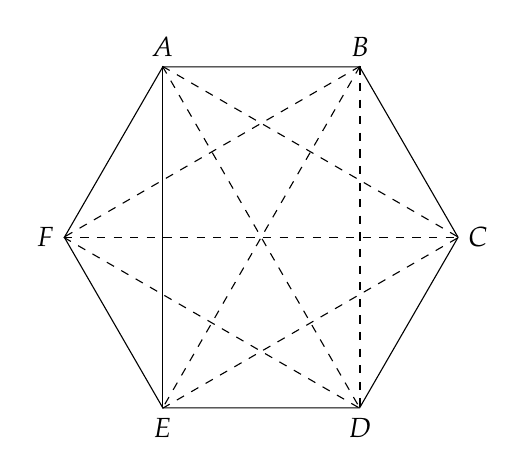
\begin{tikzpicture}
\node[name=hexagon, regular polygon, regular polygon sides=6, minimum size=5cm, draw] at (0,0) {};
\draw (hexagon.corner 2) -- (hexagon.corner 4);
\foreach \start/\finish in {1/3,1/4,1/5,2/5,2/6,3/5,3/6,4/6}
  \draw [dashed] (hexagon.corner \start) -- (hexagon.corner \finish);
\foreach \anchor/\placement/\name in {corner 1/above/$B$, corner 2/above/$A$, corner 3/left/$F$, corner 4/below/$E$, corner 5/below/$D$, corner 6/right/$C$}
  \draw (hexagon.\anchor) node[\placement] {\name};
\end{tikzpicture}

\caption{Intersecting diagonals}\label{fig.intersect}
\end{center}
\end{figure}

\item Base case: The sum of the interior angles of a triangle is $180(3-2)=180$. For the inductive step, draw a line creating an $n$-gon and a triangle. Then: $	180(n-2) + 180 = 180((n+1)-2)$. 

\item The base case, a line of length $\sqrt{1}=1$, is assumed to be given. The inductive step is shown in Figure~\ref{fig.pyth}. By the inductive hypothesis, lines of lengths $\sqrt{1}$ and $\sqrt{n}$ are constructible, and the lines can be constructed to be perpendicular. By Pythagoras's theorem, the length of the hypotenuse is $\sqrt{n+1}$.

\begin{figure}[hb]
\begin{center}
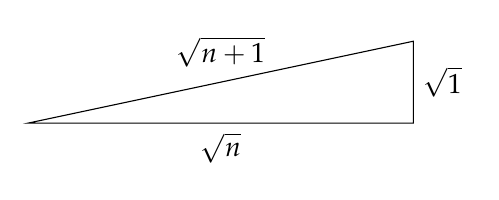
\begin{tikzpicture}
\draw (0,0) coordinate (A) -- node [above=2pt] {$\sqrt{n+1}$} (12:5) coordinate (B) -- node [right] {$\sqrt{1}$ } (B |- A) -- node [below] {$\sqrt{n}$} cycle;
\end{tikzpicture}
\caption{Constructing a line of length $\sqrt{n+1}$}\label{fig.pyth}
\end{center}
\end{figure}

\item Base case: A leaf has one node and is of height zero: $1\leq 2^{0+1}-1=1$. Inductive step: Assume that $n_h\leq 2^{h+1}-1$ and show that $n_{h+1}\leq 2^{(h+1)+1}-1$. As can be seen in Figure~\ref{fig.incomplete}, the left and right subtrees of the root are \emph{not} of the same height. However, $h+1=\max(h_l,h_r)+1$, because the height of the root is one more than the height of its subtree with maximal height. By the inductive hypothesis:
\[
\begin{array}{l}
n_l\leq 2^{h_l+1}-1\leq 2^{\max(h_l,h_r)+1}-1 = 2^{h+1}-1\\
n_r\leq 2^{h_r+1}-1\leq 2^{\max(h_l,h_r)+1}-1 = 2^{h+1}-1\,.
\end{array}
\]
Therefore:
\[
n_{h+1} = n_l + n_r + 1 \ihle{} (2^{h+1}-1) + (2^{h+1}-1) + 1 = 2^{(h+1)+1} - 1\,.
\]

\item Base case: One edge is adjacent to two nodes and there is one surface: $1+2=1+2$. There are two inductive steps: If there is a node adjacent to only one edge, remove that node and its adjacent edge. The equality $s+(n+1)=(e+1)+2$ follows from the inductive hypothesis. If there are no such nodes, then every edge is part of a cycle. Removing an edge leaves the number of nodes unchanged and reduces the number of surfaces by one. The equality $(s-1)+n=(e-1)+2$ follows from the inductive hypothesis.

%%%%%%%%%%%%%%%%%%%%%%%%%%%%%%%%%%%%%%%%%%%%%%%%%%%%%%%%%%%%%%%%%%%

\item If $n$ is divisible by $3$ we are done. Otherwise, $n=3k+1$ or $n=3k+2$. Then either $n+1=3k+2+1=3k+3$ or $n+2=3k+1+2=3k+3$ is divisible by $3$.

\item Non-inductive proof:
\begin{eqnarray*}
(x-1)\sum_{i=0}^{i=n}x^i &=& x\sum_{i=0}^{i=n}x^i - \sum_{i=0}^{i=n}x^i\\
&=&x^{n+1} + \sum_{i=1}^{i=n}(x^i-x^i) -x^0\\
&=&x^{n+1} - 1\,.
\end{eqnarray*}
Inductive proof: Base case: $x^0-1=0$, which is divisible by any polynomial. Inductive step:
\[
x^{n+1} - 1 = x^{n+1} -x^n + x^n - 1= x^n(x-1) + (x^n-1)\,.
\]
The first term is clearly divisible by $x-1$ and the second term is divisible by $x-1$ by the inductive hypothesis.

\item In the inductive step for $n+1$, we used that $a^{n}=1$ which is correct, but we also used $a^{n-1}=1$ and $a^{n-2}=1$, neither of which is correct unless we prove additional base cases $a^{-1}=1$ and $a^{-2}=1$, for all $a\geq 1$. However, both are obviously false.

\item We used the inductive hypotheses for distinct sets with $n$ elements: $s_1,s_2,\ldots,s_{n-1},s_n$ and $s_1,s_2,\ldots,s_{n-1},s_{n+1}$. However, these sets are distinct only if $n\geq 3$ and we didn't prove a base case for $n=2$. Of course that is impossible since $s_1$ might have dyed his hair green and $s_2$ might have dyed her hair blue.

%%%%%%%%%%%%%%%%%%%%%%%%%%%%%%%%%%%%%%%%%%%%%%%%%%%%%%%%%%%%%%%%%%%

\item A single literal consistent of an atomic proposition $p$ is satisfiable if and only if:
\[
A= (p \vee q \vee r) \;\wedge\; (p \vee \neg q \vee r) \;\wedge\; (p \vee q \vee \neg r) \;\wedge\; (p \vee \neg q \vee \neg r).
\]
with new atomic propositions $q$ and $r$ is satisfiable. If $p$ is assigned $T$ then $A$ evaluates to $T$. Whatever the assignments to $q$ and $r$, one of $q \vee r, \neg q \vee r,\vee q \vee \neg r, \neg q \vee \neg r$ must evaluate to $F$. If $A$ evaluates to $T$, $p$ must be assigned $T$ in the disjunction containing the literals on $q$ and $r$ that evaluate to $F$. A similar proof holds for the literal $\neg p$.

\item Let $A\stackrel{*}{\Rightarrow} w$. There are three cases depending on the first production used in the derivation. If $A \rightarrow a$, clearly, $\#a=\#b+1$ since $1=0+1$. If $A\rightarrow aS$, by the inductive hypothesis in Formula~\ref{eq.formal1}, $S\stackrel{*}{\Rightarrow} w'$ such that $\#a=\#b$ in $w'$. Therefore, $\#a=\#b+1$ in $w$. If $A\rightarrow bAA$, then by using the inductive hypothesis \ref{eq.formal2} twice, $AA\stackrel{*}{\Rightarrow} w'$ such that $\#a=\#b+2$ in $w'$, so $\#a=\#b+1$ in $w$. The proof of Formula~\ref{eq.formal3} is symmetric.

For the converse, let $S\stackrel{*}{\Rightarrow} w$ such that $\#a=\#b$ in $w$. Suppose that the first production in the derivation was $S\rightarrow aB$. Then the string $w'$ derived from $B$ has $\#a+1=\#b$. By the inductive hypothesis in Formula~\ref{eq.formal3}, there is a derivation $B\stackrel{*}{\Rightarrow} w'$, so there is a derivation $S \rightarrow aB \stackrel{*}{\Rightarrow} w$. The case where the first derivation is $S\rightarrow bA$ is similar, as are the proofs of the converses of Formulas~\ref{eq.formal2} and~\ref{eq.formal3}.

%%%%%%%%%%%%%%%%%%%%%%%%%%%%%%%%%%%%%%%%%%%%%%%%%%%%%%%%%%%%%%%%%%%

\item Lemma 2: For all $i$, the sequence of elements in $B_i$ is ordered \emph{and} all elements in $A_i$ are greater than or equal to all elements in $B_i$.

Base case: $B_0$ is empty so the claims are vacuous. Inductive step: The inductive hypothesis that Lemma 2 holds for $A_i$ and $B_i$. Therefore, the element $a_i$ added to the end of $B_i$ to form $B_{i+1}$ is greater than or equal to all elements in $B_i$, so $B_{i+1}$ is ordered. All elements of $A_{i+1}$ are greater than or equal to all elements in $B_{i+1}$: (1) by the inductive hypothesis they were already greater than or equal to all elements in $B_i$, and (2) $a_i$ was the smallest element of $A_i$ so they are also greater than or equal to $a_i$ which was added to $B_i$ to construct $B_{i+1}$.

\item Base case: the variable \texttt{sem} is initialized to $1$ and $\#\mathit{CS}=0$ since no process is in its critical section. By the inductive hypothesis assume that the formula is true. It can be falsified only if the values of $\#\mathit{CS}$ or $\mathit{sem}$ change. The two processes are symmetric so without loss of generality this can happen only upon executing \texttt{p1} or \texttt{p3}. Executing \texttt{p1} increases $\#\mathit{CS}$ by $1$ but also decreases $\mathit{sem}$ by $1$. Similarly, executing \texttt{p3} decreases $\#\mathit{CS}$ by $1$ but also increases $\mathit{sem}$ by $1$. 

%%%%%%%%%%%%%%%%%%%%%%%%%%%%%%%%%%%%%%%%%%%%%%%%%%%%%%%%%%%%%%%%%%%

\item If $n$ is odd, $n-7$ is even, so if we can construct arbitrary large even numbers, we can construct arbitrary large odd numbers by adding one $\$7$ coin. Clearly, if $n=4k$, $n$ can be constructed from $k$ $\$4$ coins. So all we have to prove is that an even number not divisible by $4$ can be constructed.

It is easy to show that the numbers $1,2,3,5,6,9,10,11,13,15,17$ cannot be constructed. For example, $17$ is odd so a $\$7$ coin must be used and it can be used only once because $17-2\cdot 7=3$ cannot be constructed. But $17-7=10$ is not divisible by $4$ so it is not constructible. We now prove by induction that even numbers greater $\geq 18$ and not divisible by $4$ are constructible.

Base case: $18=2\cdot 7 + 4$.

Even numbers not divisible by $4$ can be expressed as $2(2k+1)$. Inductive step:
\[
2(2(n+1)+1) = 4n+6 = (4n+2)+4.
\]
By the inductive hypothesis, $4n+2=2(2n+1)$ can be constructed. Adding one $\$4$ coin constructs $2(2(n+1)+1)$.

\item The base case is when $\frac{a}{b}$ is itself a unit fraction, $a=1$. The inductive hypothesis is that the claim is true for all fractions less than $\frac{a}{b}$. By the inductive hypothesis and the choice of $\frac{1}{q} < \frac{a}{b}$,
\[
\left( \frac{a}{b} - \frac{1}{q} \right) < \frac{a}{b}
\]
can be expressed as a sum of unit fractions; therefore:
\[
\frac{a}{b} = \frac{1}{q} + \left( \frac{a}{b} - \frac{1}{q} \right)
\]
can be expressed as a sum of unit fractions.

If $\frac{1}{q}$ is the \emph{largest} unit fraction less than $\frac{a}{b}$, then $\frac{a}{b} < \frac{1}{q-1}$, so $aq-b < a$, and:
\[\left( \frac{a}{b} - \frac{1}{q} \right) = \frac{aq-b}{bq} = (aq-b)\cdot \frac{1}{b}\cdot\frac{1}{q} < a\cdot\frac{1}{b}\cdot\frac{1}{q}<\frac{1}{q}\,,
\]
since $\frac{a}{b}$ is a proper fraction. Therefore, none of the unit fractions in the sum expressing $\left( \frac{a}{b} - \frac{1}{q} \right)$ can be greater than or equal to $\frac{1}{q}$.

\item Let us first prove that $\phi^2=\phi+1$:
\vspace*{-8pt}
\begin{eqnarray*}
\phi^2 &=& \left(\frac{1+\sqrt{5}}{2}\right)^2\\
&=& \frac{1}{4} + \frac{2\sqrt{5}}{4} + \frac{5}{4}\\
&=& \frac{2}{4} + \frac{2\sqrt{5}}{4} + \frac{4}{4}\\
&=& \frac{1+2\sqrt{5}}{2} + 1\\
&=&\phi + 1\,.
\end{eqnarray*}
The proof that $\bar{\phi}^2=\bar{\phi}+1$ is similar.

The base case for $n=1$ is:
\[
\frac{\phi^1 - \bar{\phi}^1}{\sqrt{5}}=\frac{(1+\sqrt{5})/2-(1-\sqrt{5})/2}{\sqrt{5}}=\frac{2\sqrt{5}}{2\sqrt{5}}=1\,.
\]

Assume the inductive hypothesis for all $k\leq n$. The inductive step is:
\begin{eqnarray*}
\phi^n - \bar{\phi}^n &=& \phi^2\phi^{n-2} - \bar{\phi}^2\bar{\phi}^{n-2}\\
&=&(\phi+1)\phi^{n-2} - (\bar{\phi}+1)\bar{\phi}^{n-2}\\
&=&(\phi^{n-1} - \bar{\phi}^{n-1}) + (\phi^{n-2} - \bar{\phi}^{n-2})\\
&\ih&\sqrt{5}f_{n-1} + \sqrt{5}f_{n-2}\,,
\end{eqnarray*}
so:
\[
\frac{\phi^n - \bar{\phi}^n}{\sqrt{5}} = f_{n-1} + f_{n-2} = f_n\,.
\]

\newpage

\item Proof of Pascal's rule:
\begin{eqnarray*}
{n \choose k} + {n \choose k+1} &=& \frac{n!}{k!(n-k)!} + \frac{n!}{(k+1)!(n-(k+1))!}\\
&=&\frac{n![(k+1)+(n-k)]}{(k+1)!(n-k)!}\\
&=&\frac{n!(n+1)}{(k+1)!(n-k)!}\\
&=&\frac{(n+1)!}{(k+1)!((n+1)-(k+1))!}\\
&=&{n+1 \choose k+1}\,.
\end{eqnarray*}

The base case is:
\[
f_1 = 1 = {1 \choose 0} = \frac{1!}{0!(1-0)!}\,.
\]

The inductive step is:
\begin{eqnarray*}
f_{n-1} + f_{n-2} &\ih& {n-1 \choose 0} + {n-2 \choose 1} + {n-3 \choose 2} + {n-4 \choose 3} + \cdots\\
&&\hspace{5em}{n-2 \choose 0} + {n-3 \choose 1} + {n-4 \choose 2} + \cdots\\
&=&{n-1 \choose 0} + {n-1 \choose 1} + {n-2 \choose 2} + {n-3 \choose 3} + \cdots\\
&=&{n \choose 0} + {n-1 \choose 1} + {n-2 \choose 2} + {n-3 \choose 3} + \cdots.
\end{eqnarray*}
The last equality uses ${k \choose 0} = \frac{k!}{0!(k-0)!} = 1$ for any $k$.

\end{enumerate}

\end{document}
